\chapter{Technical Background}
\label{lab:technical}

\section{Terms and Definitions}
\label{sec:terms}

A Web server can be utilised to handle rather different tasks, from merely delivering static assets like images to serving entire Web pages to representing a service endpoint communicating with a range of different devices. This section aims to give an overview of the basic requirements a modern Web server architecture needs to fulfil. Moreover, important performance factors are elaborated with regard on high-demand and high-performance setups.

\subsection{Network Communication}
The eponymous task of a Web server is to serve Web-connected clients over the medium of the Internet. This involves receiving and sending messages using different implementations of network protocols. The most widely used protocol of the Web, \textit{HTTP}\footnote{Hypertext Transfer Protocol}, is a request-response protocol, which means that for every message a client sends to a server, a response is sent back \cite{http}. To minimise networking latency, it is preferable for a Web server to have a high-speed connection to the Internet, fast system I/O\footnote{\label{lab:io}Input and Output, esp. hardware} and capable routing hardware. However, these parameters are not directly related to software and are thus neglected during the further course of this thesis.

\subsection{Dynamic Content}
Originally, the Web was intended to be a network of interconnected text files, which later were augmented with images and custom styles; Web servers were basically required to understand incoming requests and respond by streaming the right static content back to the client \cite{http}. With the release of \textit{PHP}\footnote{Recursive acronym: PHP Hypertext Preprocessor, \url{http://php.net/}}, \textit{ASP}\footnote{Active Server Pages, \url{http://msdn.microsoft.com/en-us/library/aa286483.aspx}} and \textit{Java}\footnote{\url{https://www.java.com/}} in 1995, 1996 and 1997, respectively, webpages that are prepared by the server based on dynamic data -- like database content or user input -- became widespread \cite{webhistory}. From that point on, Web servers needed more processing capabilities for script execution and database access; however, the number of requests remained roughly the same \cite{webhistory}.

\subsection{Asynchronous Requests}
The advent of \textit{AJAX}\footnote{Asynchrounous JavaScript and XML (Extensible Markup Language)} and mobile applications in the late 2000's changed requirements drastically. Rather than requiring to refresh the whole view for every piece of information sent and received, data could now be transferred programmatically in the background. By asynchronously communicating with an API\footnote{Application Programming Interface, an interface for connecting different applications at code-level.} endpoint, operations like deleting an item from a list could be performed ubiquitously without reloading the page context. Especially applications that aim to provide desktop-like behaviour and capabilities -- commonly called Rich Internet Applications -- make heavy use of asynchronous requests \cite[p. 4]{Sencha2011}. This also changed users' expectations for websites from anticipating a certain amount of load time to implicating real-time behaviour \cite{Garrett2005}. To achieve low latency while maintaining client-server information consistency, the server's performance had to meet the combined request frequency of all clients.

\subsection{Request Frequency and Response Time}
\label{lab:frequency}
Since in many cases the responsiveness of the user interface -- and with it the user experience -- depends on the duration of the server communication roundtrip, maintaining acceptable response times is often crucial \cite[p. 1]{Nadimpalli2000}. Request frequency and response time correlate in the sense that request frequency represents the demand on a server endpoint while response time -- given equally demanding operations per request -- can be interpreted as the potential of the server to meet the demand. When the processing limit of the server is met, response times generally become inversely proportional to the request frequency (see figure \ref{fig:response_time}) \cite{response_time}. At this point, the server may neglect the request (ideally indicated by returning an error response to the client), not respond at all or even stop serving clients altogether (i.e. ``crash'') \cite{http}.

\begin{figure}
\centering\small
\setlength{\tabcolsep}{0mm}
  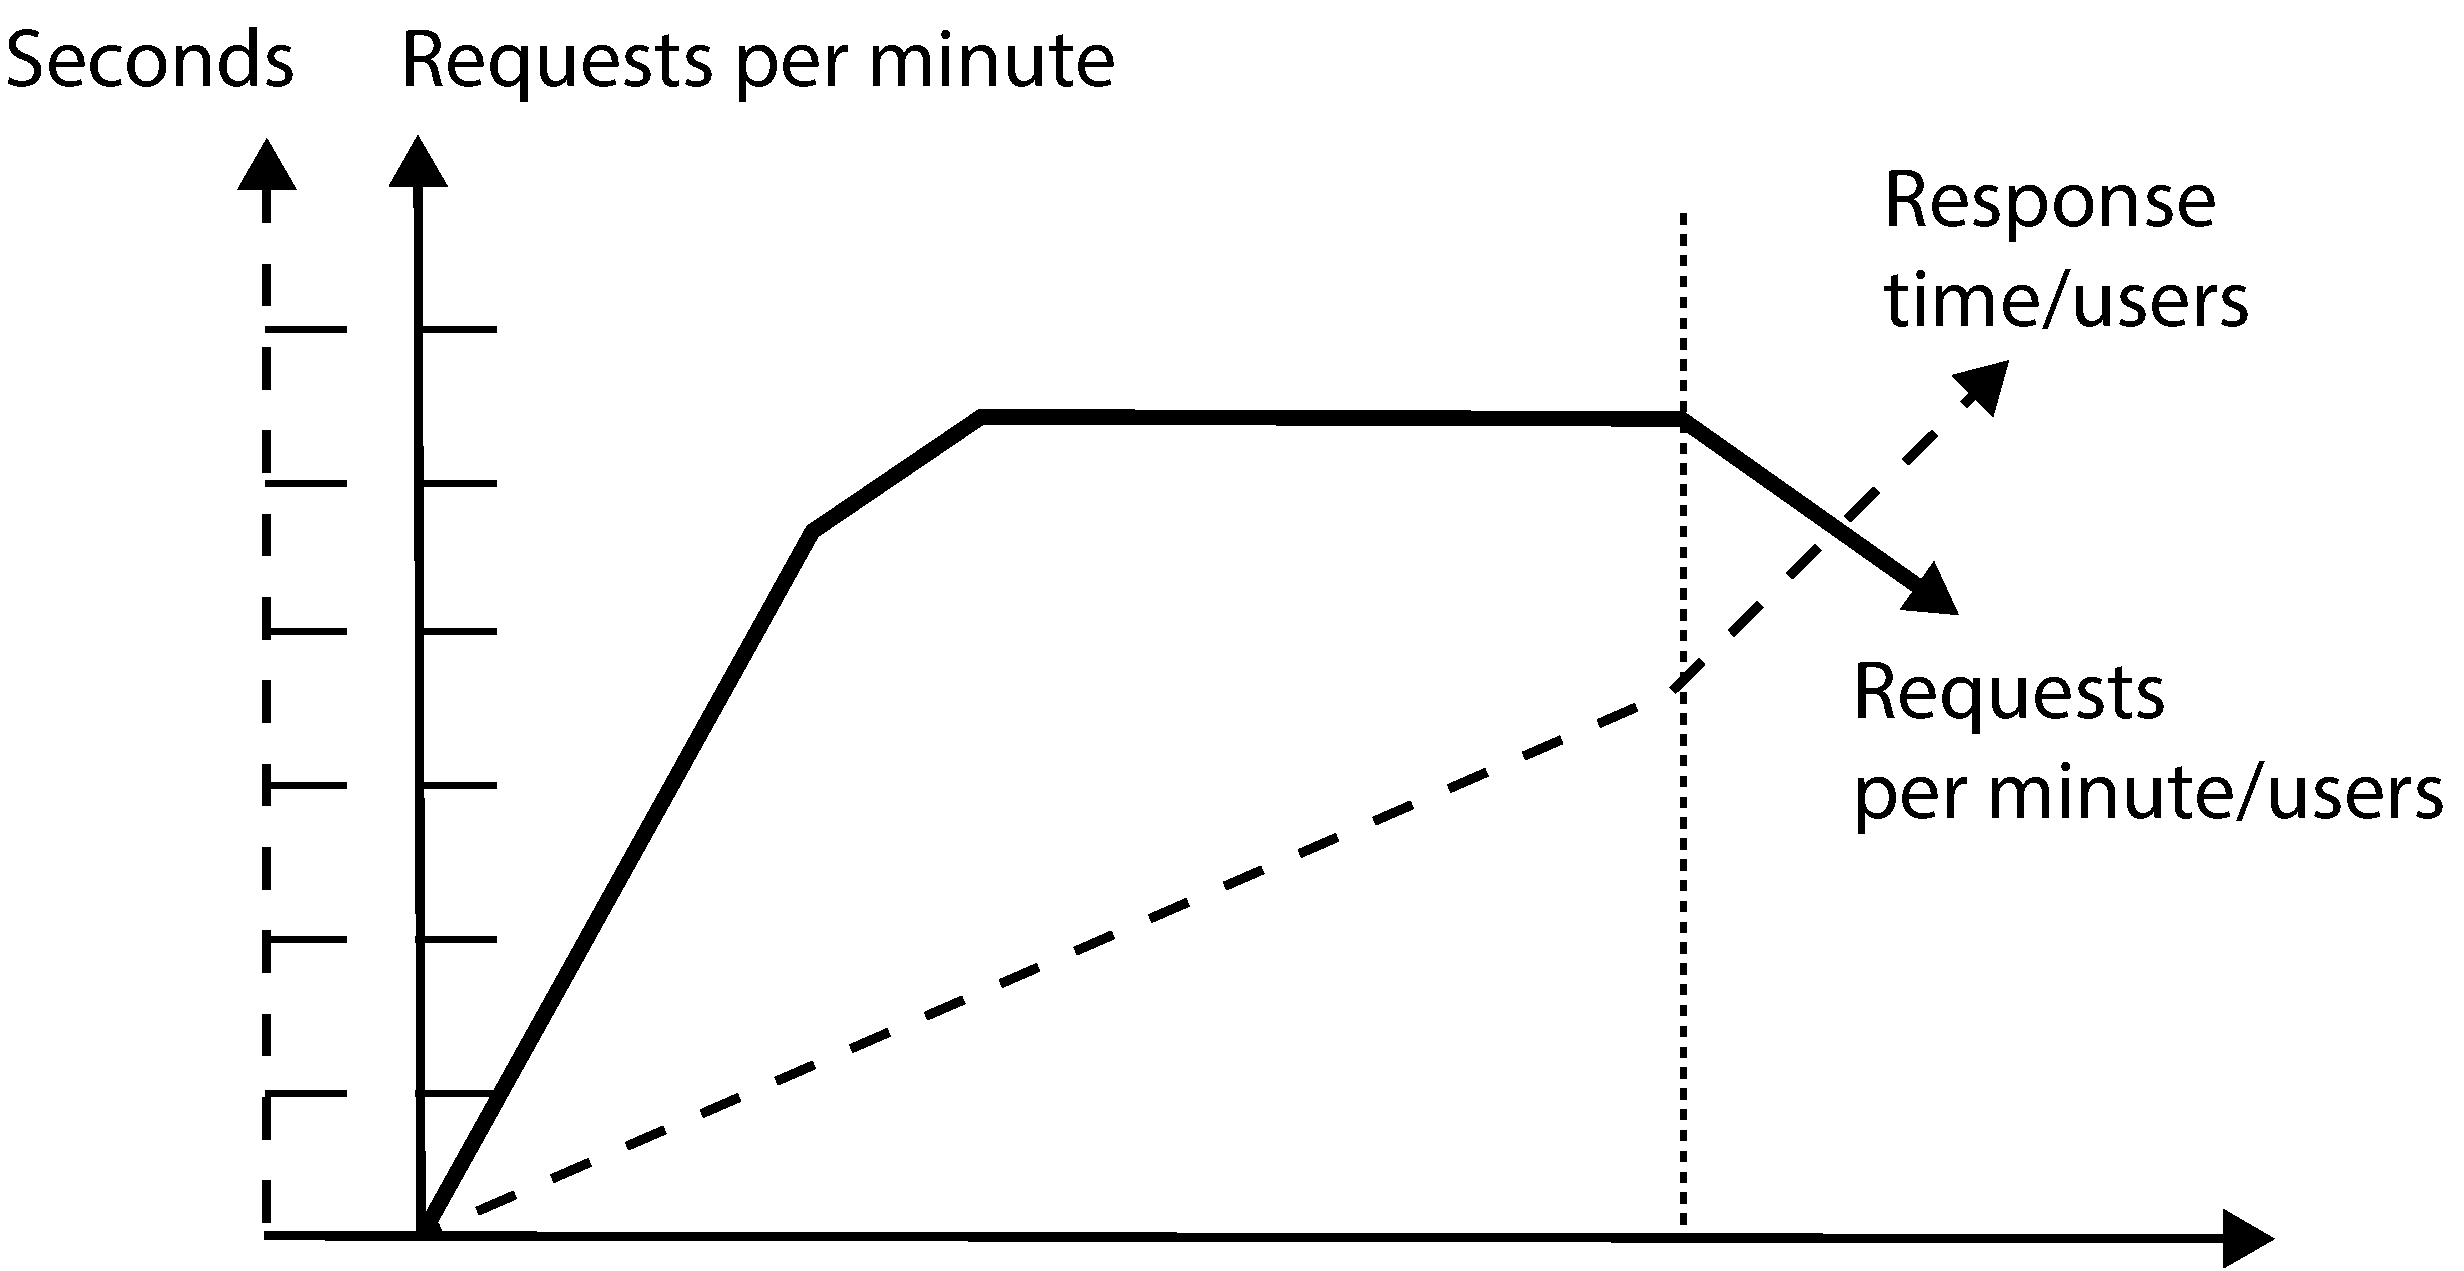
\includegraphics[width=.80\textwidth]{response_time}
\caption{
Correlation between request frequency and response time in a typical Web server setup. After the server has reached its limit of linearly serving clients (indicated by the dotted line), response times become inversely proportional to the request frequency. Image source: \cite{response_time}
}
\label{fig:response_time}
\end{figure}

\subsection{Scalability}
Demands on Web servers typically are lower during the initial phase of a business and grow with the popularity of the service. Since business growth and server load can not be exactly predicted, it is necessary to be able to adjust (i.e. \textit{scale}) the entire server architecture according to current needs in a timely manner. The \textit{Slashdot Effect} describes a sudden rise or spike in service popularity and can -- due to the open nature of the Web -- lead to a tremendous increase in activity over a relatively short timespan \cite[p. 1]{Drolia2010}. 

Today's hardware is well suited to meet high demands and can be configured flexibly: If a larger number of physical server units as well as the necessary infrastructure is available, requests can be distributed across different systems and the load a single unit has to handle decreases. If single units are outfitted with more memory and faster processors, the number of request operations one unit can process increases. Since acquiring and maintaining server units and other infrastructure components is expensive, well-designed software can make a significant difference in system efficiency, which in turn can greatly benefit any business -- especially with the \textit{pay-what-you-use} model modern service providers offer\footnote{So-called \textit{Cloud} service provider often offer flexible plans on processing power, that can be dynamically adjusted without significant server down-time.} \cite[p. 11]{Hughes-Croucher2012}. Software that is well-suited to be expanded according to its usage is considered \textit{elastic} \cite{reactive}.

Ideally, the server software should be hardware agnostic, i.e. should behave consistently independent of the hardware it runs on. For instance, if the software depends heavily on sharing application state via RAM\footnote{Random Access Memory}, scaling out on more than one machine will be unsuccessful \cite{Veal2007}. Scalability can be measured by the relationship between hardware resources and the increase of performance. If this relationship is nearly linear, the system is considered to scale well.

\subsection{Development}
Not a part of the production system itself, but nonetheless an essential part of all Web server applications is their development. A structured, idiomatic way of writing application logic doubtlessly contributes to every software product. Modularisation of components facilitate the use of third-party software like libraries and frameworks. In return, using existing software products can greatly reduce development time and effort, while simultaneously providing robust, tested solutions. Web server applications particularly benefit from frameworks since they often handle standard, repetitive tasks like network I/O\footnoteref{lab:io}, database access and caching \cite[p. 1]{Reelsen2011}. Integrating and maintaining these frameworks is a major part in implementing a Web server application; thus, not only the performance, but also the ease of use of Web frameworks and their language environments are important criteria.


\section{Concurrency Models}
\label{sec:concurrency}

Since a Web application in a production setting is usually publicly accessible, serving multiple clients simultaneously is the rule, rather than the exception. Depending on the popularity of the service, the number of concurrent requests can range anywhere from dozens to several thousands, e.g. for social media sites \cite[p. 1]{Drolia2010}. A server process with a single flow of control would only be able to serve one client at once, with all requests received while the server is busy being neglected. Therefore, networking applications always have to be implemented using multiple program flows that can be executed concurrently \cite{Webopedia}. This section lists various paradigms associated with designing an application capable of maintaining multiple flows of control.

\subsection{Purely Thread-based Model}
\label{sec:threads}
A thread is a sequence of instructions within a program. Allocating processing time to threads is handled by an operating system scheduler. To have a program execute multiple logic structures concurrently, they have to be explicitly abstracted in the form of threads. Physical concurrency occurs, when threads are executed simultaneously -- i.e. at the exactly same time -- on different processor cores; in contrast, logical concurrency describes that multiple threads are executed sequentially in rapid succession at roughly the same time, thus giving the impression of simultaneous execution. Physical concurrency is inherently more efficient \cite{ThreadsJava}.

\subsubsection*{Flow of Control}
A great advantage of threads in the context of Web server applications lies in the natural abstraction level regarding multiple parallel requests: Client communication is commonly treated as a set of mutually independent connections; this approach of abstraction facilitates a clear program flow structure \cite{Veal2007}. According to this model, every request can be treated as an isolated flow of control (see figure \ref{fig:thread_server}). However, since threads are not isolated from each other and share state via a common memory address space, this only holds true as long as resources like queues or caches are accessed sequentially \cite[p. 2]{Behren2003}. Thus, developers have to pay close attention to avoid race-conditions, deadlocks and access violations -- complications that generally result from improper thread coordination or application design \cite[p. 1]{Fischer2007}. Therefore, the implementation of large-scale systems heavily relying on threads always introduces additional complexity \cite[p. 1]{Lee2006}.

\begin{figure}
\centering\small
\setlength{\tabcolsep}{0mm}
  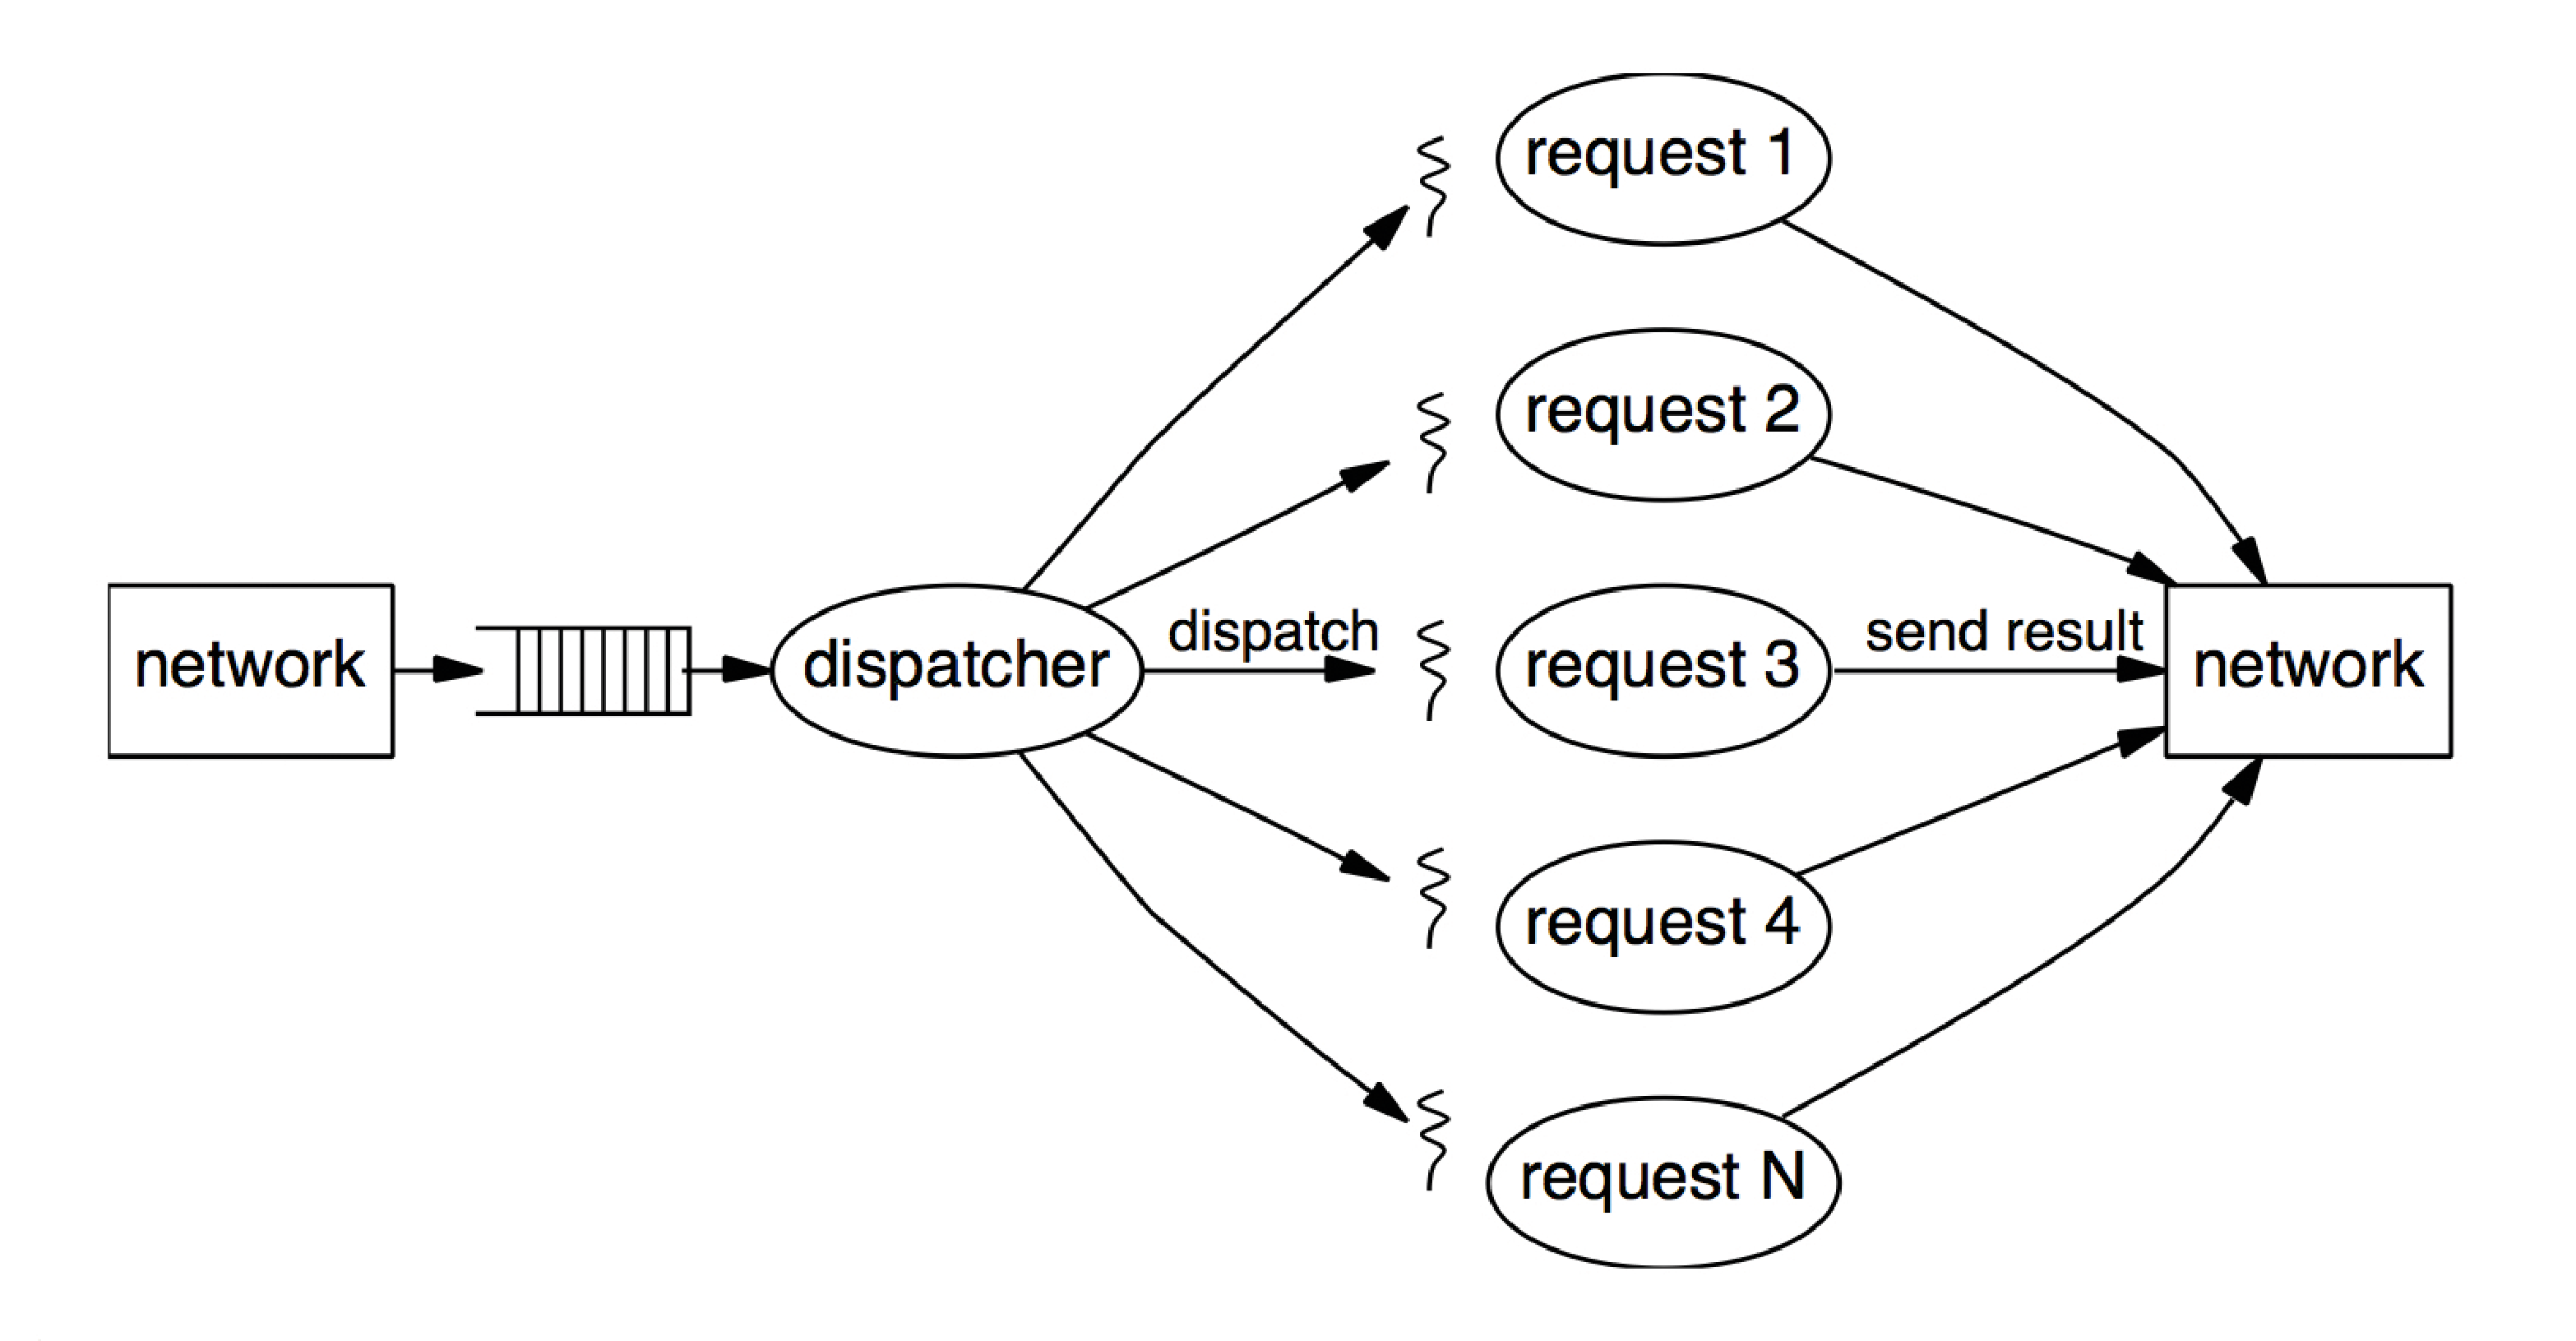
\includegraphics[width=.90\textwidth]{thread_server}
\caption{
On a purely thread-based Web server, each request is handled by a dedicated thread. Incoming network requests are queued and sequentially accepted by a dispatcher, that distributes them among available threads -- either by using idle threads from a thread pool or by creating new threads. Image source: \cite{Welsh2001}
}
\label{fig:thread_server}
\end{figure}

\subsubsection*{Scalability}
Traditionally, Web server applications process each request on a dedicated thread throughout its whole lifespan, from accepting it to responding to it \cite[p. 162]{Henderson2006}. This behaviour can be observed for instance in implementations of the popular LAMP\footnote{Linux, Apache, MySQL, PHP} server stack configuration \cite[p. 48]{Henderson2006}. A less experienced programmer might find this ideal, since concurrency stays mostly hidden and the application logic is based solely on the flow of a single request -- smaller projects might not expose any drawbacks of this setup at all. However, it is obvious, that to scale up a thread-based system, the number of threads has to be increased. The number of threads engaging in simultaneous processing, i.e. physical concurrency, is limited by the number of processing cores. This means that on a computer equipped with a quad-core processor, four threads can be executed -- and thus, four requests can be served -- in parallel\footnote{\label{lab:hyper}Certain implementations of simultaneous multithreading allow for increasing this number at the cost of reduced performance per thread, for instance Intel's Hyper-Threading Technology (\url{http://www.intel.com/)}.}.

\subsubsection*{Drawbacks}
Problems arise when a thread has to wait for another requirement to be fulfilled. The process of meeting a requirement that renders the executing thread unable to proceed is called a \textit{blocking} operation. Such actions include for instance reading or writing a file on disk, handling network traffic or file uploads, querying a database, accessing another Web service or processing intensive computations \cite[p. 196]{Henderson2006}. When a thread encounters a blocking operation, it cannot advance further in the program flow until the operation completes (see figure \ref{fig:concurrency_1}). The resulting delay can account to anywhere from a few milliseconds to several seconds, for instance when accessing a slow or unresponsive Web service. The only way to counteract the temporary occupation of threads and to continue processing incoming requests is the creation of new threads \cite[p. 36]{Hughes-Croucher2012}. However, every newly created thread counts towards certain limitations in scalability. On the one hand, every thread receives a predefined share of process address space memory -- also known as \textit{stack} -- upon creation to temporarily store data \cite{Russinovich}; since memory is reserved in advance without knowing the exact requirements of the thread, a certain amount of memory overhead is likely. On the other hand, the entirety of all threads has to be orchestrated by an operating system module called \textit{scheduler}, which requires processing time relative to the number of threads \cite{Russinovich}. Moreover, a computationally expensive procedure called \textit{context switching} must also be followed upon changing the actively processed thread \cite{threads_vs_events}. This process includes complications called \textit{buffer} and \textit{cache misses} as well as lock contentions \cite[p. 2]{Welsh2001}. When a certain number of active threads is reached, this can lead to serious performance degradation, as illustrated in figure \ref{fig:thread_scale}. Especially when the application is executed inside a \textit{virtual machine}\footnote{A software-based emulation of a computer, that executes programs like a physical machine.} -- which is often the case for distributed applications due to better replicability -- the over-provisioning of memory leads to scarce resources \cite[p. 1]{Haller2006}.

\begin{figure}
\centering\small
\setlength{\tabcolsep}{0mm}
  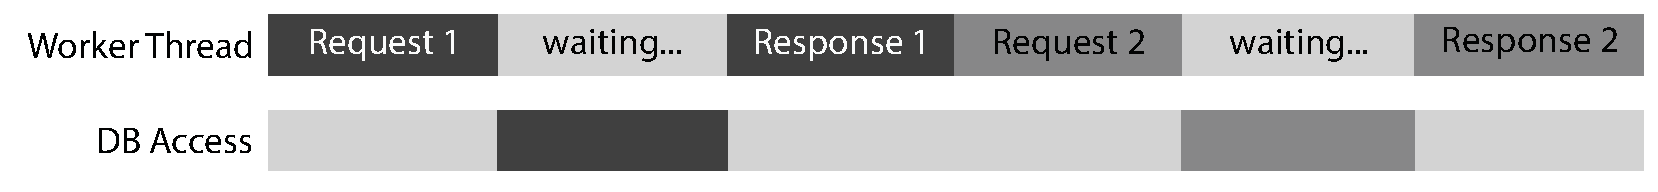
\includegraphics[width=.90\textwidth]{concurrency_1}
\caption{
A typical blocking situation in Web server scenario. When request one (shown in dark grey) arrives, a database operation is necessary. During the course of this operation, the executing thread blocks while waiting for results. The response can only be sent when data is returned and the next request (shown in medium grey) can only be served after the first one completes.
}
\label{fig:concurrency_1}
\end{figure}

\begin{figure}
\centering\small
\setlength{\tabcolsep}{0mm}
  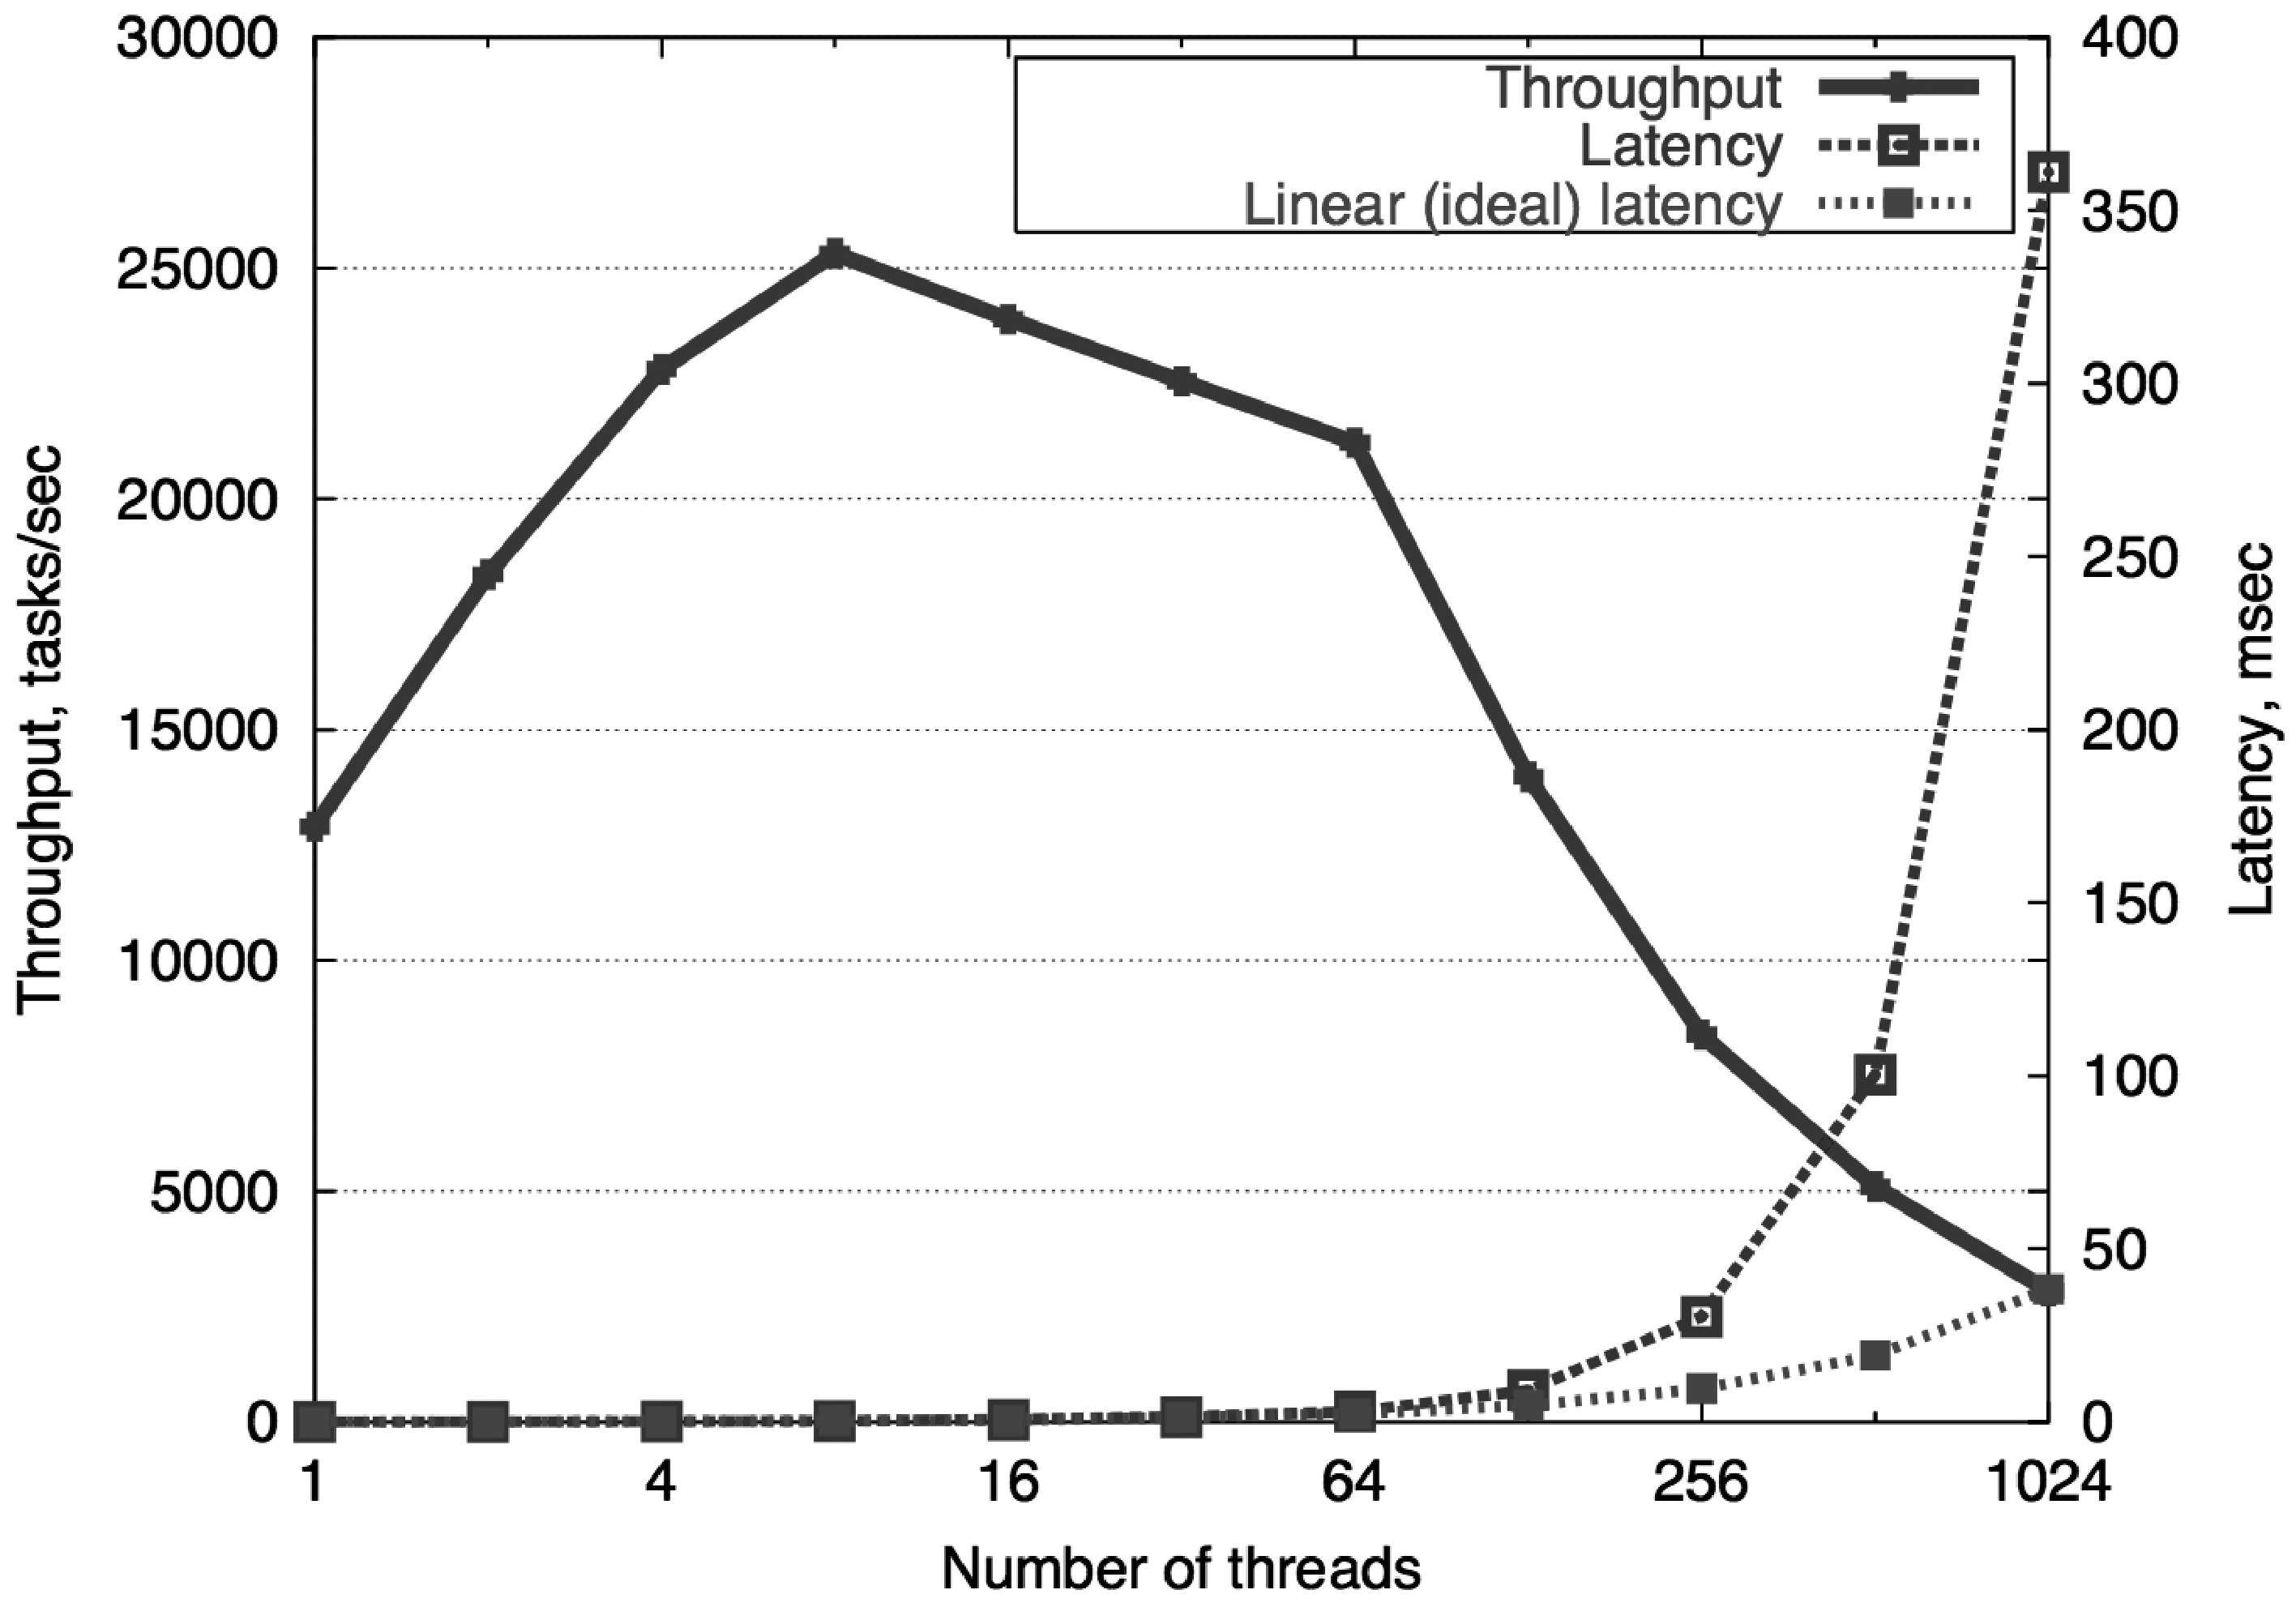
\includegraphics[width=.90\textwidth]{thread_scale}
\caption{
This graph shows the performance degradation resulting from rising request frequency for a purely thread-based Web server. Because of the performance overhead introduced by a large number of concurrent threads, the processing throughput decreases. If the number of threads grows above a certain point, the response time escalates due to the shortage of resources. The data is taken from an experiment by M. Welch et al. \cite{Welsh2001}. Image source: \cite{Welsh2001}
}
\label{fig:thread_scale}
\end{figure}

Some of the problems of threads can be addressed by using a \textit{thread pool}: Instead of spawning new threads upon each request, a fixed number of threads is spawned in advanced and workload is distributed among them. However, this procedure is not without problems and introduces the delicate step of setting the thread pool size \cite{threadpools}. It can be concluded that a lower thread overhead can benefit the overall performance of a process. Furthermore, when scaling an application, the maximum number of simultaneously processed threads can at best increase linearly in relation to the number of processing cores in a system \cite{McCool}.

\subsection{Event-based Model}
\label{lab:events}
While threads on their own present a convenient abstraction for handling Web requests, recent years have seen an incline towards event-driven architectures \cite{Tilkov2010}. Events can be seen as an arbitrary change in application state; an example of an event may be an arriving HTTP request. An event is often abstracted to an object that is passed along with the flow of control and may consist of a header describing its nature (e.g. the fact that it represents an HTTP request) and a body containing additional information (e.g. request parameters and client identification). A different part of the application may subsequently \textit{react} to this event by executing further operations like querying the database.

Using events is a significant departure from the traditional \textit{command-and-control} style used for instance in purely thread-based architectures (see section \ref{sec:threads}). However, seen from a different perspective, using events on a Web server is at least as idiomatic as using threads; the Web server has no control over the arriving requests, yet it has to respond by executing application logic. Instead of forcefully maintaining control over the execution context, the Web server may also relinquish control and let itself be controlled by events. This strategy follows the principle of \textit{inversion of control} \cite{Hohpe2006}. 

Event-driven programming does not preclude the existence of threads; neither is it the opposite or an evolutionary step. All major operating systems use threads as a means of managing process execution; thus, even a purely event-driven program runs at least on one thread.

\subsubsection*{Flow of Control}
\label{lab:flow}
While event-driven programming does not imply a certain concurrency model, the employed concepts have a strong influence on how concurrency is handled by the application. This section elaborates the basic concepts of event-driven programming.

At its simplest, an event-driven application consists of two major components: On the one hand an \textit{event loop} containing an \textit{event listener} and on the other hand an \textit{event handler}. The event loop is a lightweight structure passing incoming events from a queue to event listeners that have subscribed to a certain kind of event, e.g. an incoming network request. The targeted event listener then passes the event on to a handler function, which executes application logic and may create another event upon completion. Larger applications typically have one event loop per process and a number of listeners and handlers (see figure \ref{fig:event_loop}) \cite[p. 33]{Hughes-Croucher2012}.

\begin{figure}
\centering\small
\setlength{\tabcolsep}{0mm}
  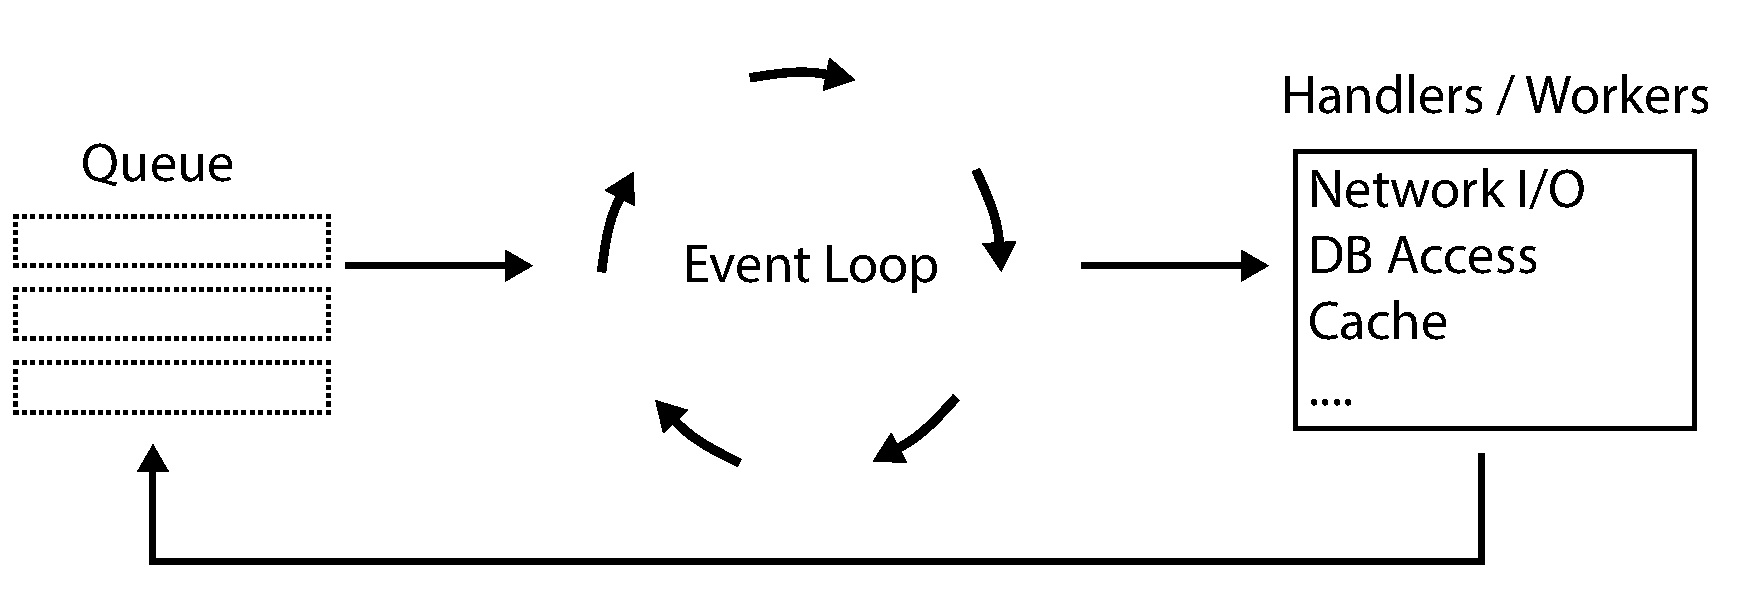
\includegraphics[width=.80\textwidth]{event_loop}
\caption{
Basic flow of control in an event-driven application. Operations that would normally block the event loop are executed separately and create further events upon completion.
}
\label{fig:event_loop}
\end{figure}

The use of events leads to an inherently \textit{flat} application structure in the sense that there is no hierarchical ordering of event sources and destinations. There are two ways of advancing in the flow of control at the end of a particular operation: The first option is to create a new event that is received by the event loop and propagated to the next event handler. The second way is to employ a \textit{callback function}. Calling a callback function can be regarded as transferring the flow of control to an event handler without consulting the event loop \cite[p. 92]{Erb2012}. Callback functions are often used to handle results of a blocking operation -- like making a request to a remote Web service -- directly upon its completion and thus maintaining control over the execution order of further actions. Implementation is typically done via either a function pointer or an \textit{annonymous function}, as demonstrated in program \ref{prog:callback}.

\begin{program}
  \caption{Calling a callback function via a function pointer (above) and via an annonymous function (below) in JavaScript. The request to a Web service may take some time and is thus executed asynchronously. When the response from the service arrives, the callback is executed. For this example, the response is printed to the console, which is a rather fast action and therefore can be executed in a blocking fashion.}
  \label{prog:callback}
  \begin{JavaCode}
function callbackFunction (data) {
    console.log(data);
}
  
WebService.get("http://example.com/").then(callbackFunction);
  \end{JavaCode}
\begin{JavaCode}
WebService.get("http://example.com/").then(function(data) {
    console.log(data);
});
  \end{JavaCode}
\end{program}

Neither events nor callback functions are usually found in traditional -- i.e. sequential -- programming. In nearly all application environments, the default way of executing routines in succession is to use functions, which return values that are used during the further course of the program. This proven concept determines three major aspects of program flow \cite[p. 3]{Hohpe2006}:

\begin{description}
  \item[Coordination] The ordered execution of sequential operations, which prevents problems associated with concurrency
  \item[Continuation] The program flow continues immediately after the function call, thus eliminating the need to explicitly define a continuation point
  \item[Context] The proper handling of the local variable scope; if a function returns, the previous context is restored and the callee function can use the same variable scope as before the calling operation  
\end{description}

\begin{figure}
\centering\small
\setlength{\tabcolsep}{0mm}
  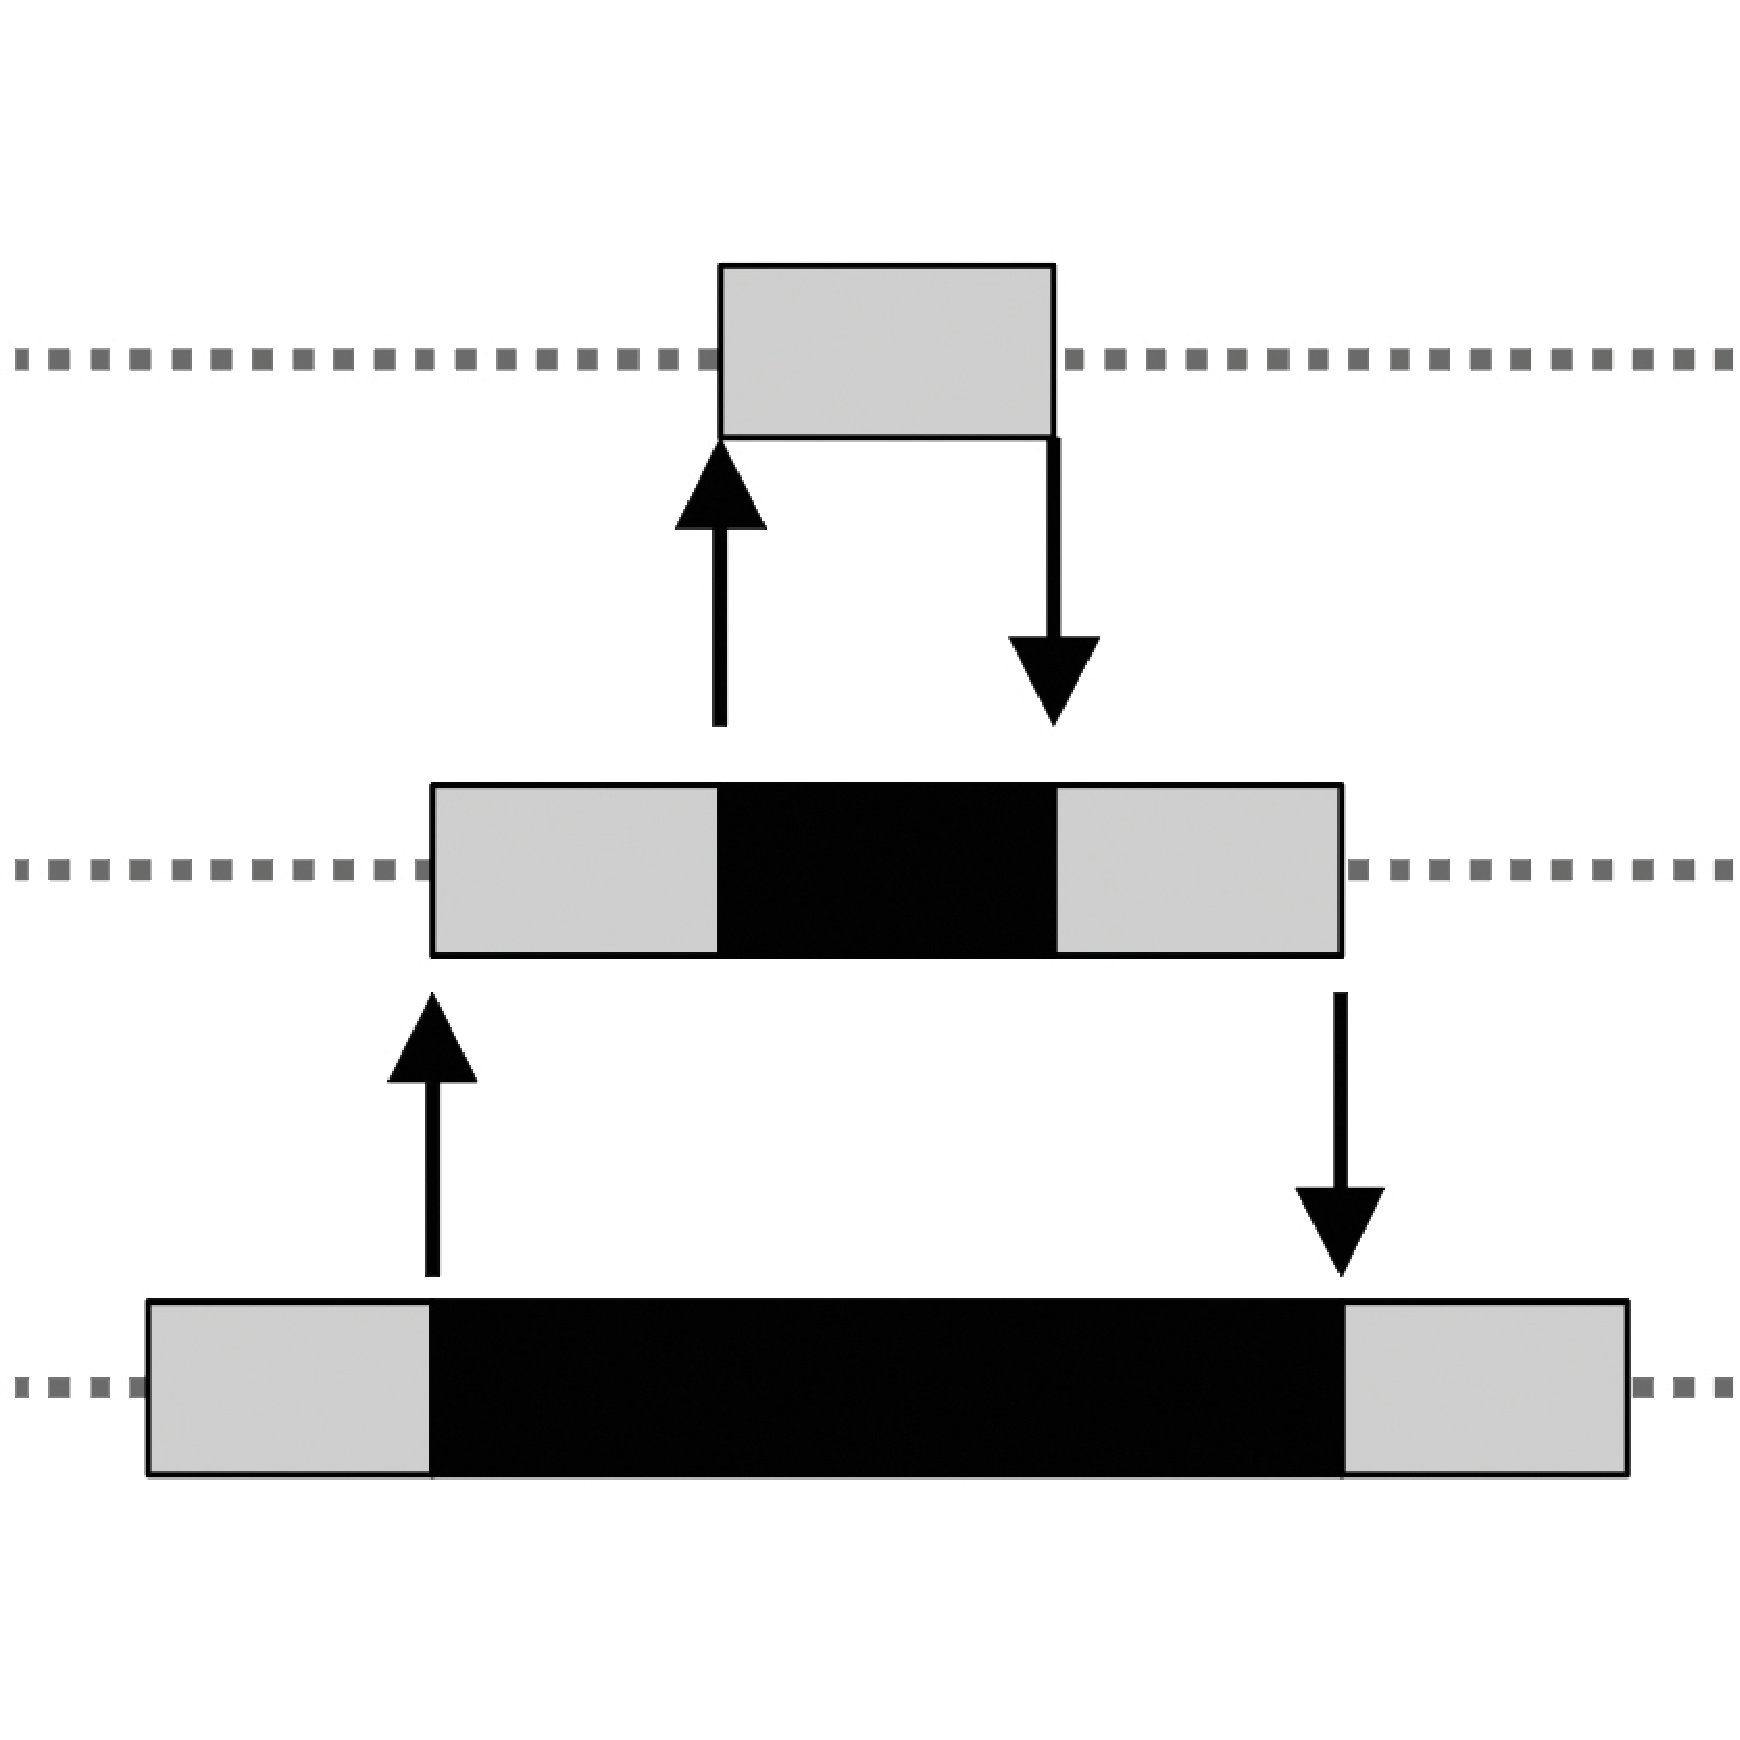
\includegraphics[width=.50\textwidth]{stack}
\caption{
Illustration of a simple call stack structure. As time progresses (horizontal axis, left to right), the call stack grows with each function call. As the functions return gradually, the stack size decreases again. Active parts of functions are shown in grey, passive (i.e. ``waiting'') parts are shown in black. Image source: \cite{Hohpe2006}
}
\label{fig:stack}
\end{figure}

To store the references and contexts of all functions during such a succession of calls, a dedicated part of memory called the \textit{call stack} is used (see figure \ref{fig:stack}). Despite its advantages, heavy use of the stack in the context of modern Web applications poses two substantial problems: On the one hand, the concept of the stack origins from a time where concurrent computing was not frequently used -- especially in the manner seen in highly concurrent applications. The behaviour of the stack pursues a strongly linear manner of execution. Because at any point in time, only one call can be pushed onto the stack at once, only one action can happen at a time. Likewise, if an operation were to take an extended or unspecified period of time -- like accessing a remote Web service -- a single call stack provides no way of executing another operation during this time. The second problem of the call stack is that it can not be distributed across physically or logically separated systems. Pushing a call onto the stack implies that a return memory address -- i.e. a continuation point -- is known and clearly specified, which is not the case for distributed systems \cite{Hohpe2006}. 

The departure from the stack also implies a concept called \textit{loose coupling}. This means, that the components of interaction within a program do not need to know the exact specifications of the target. One example would be a new user registering for the service: A tightly coupled system would need to call the exact function that creates the user in the database. In an event-based system an event called \texttt{userCreated} (or similar) would be created and the database component would receive this event. This leads to a more flexible and resilient application structure, because changes to the exact implementation of one component do not require changes on the other side. The act of developing an application without a call stack is known as \textit{stack ripping} \cite{Drolia2010}.

\subsubsection*{Scalability}
In contrast to the purely thread-based concept presented in section \ref{sec:threads}, event-based architectures tend to scale better. One major reason for this is the blocking behaviour of the I/O thread; while in purely thread-based systems the thread accepting an incoming request is no longer available for processing until all blocking operations have finished, the I/O thread in event-based systems only processes short-lived operations. Thus, in the latter, scalability is not directly proportional to the number of threads used by the system (see figure \ref{fig:events_scale}) \cite[p. 2]{Carrera}. Furthermore, because the execution context of event-based program flow is event-specific, global context switching can be minimised. This leads to an increased actual concurrency of executed program code compared to purely thread-based systems \cite{Lee2006}.

\begin{figure}
\centering\small
\setlength{\tabcolsep}{0mm}
  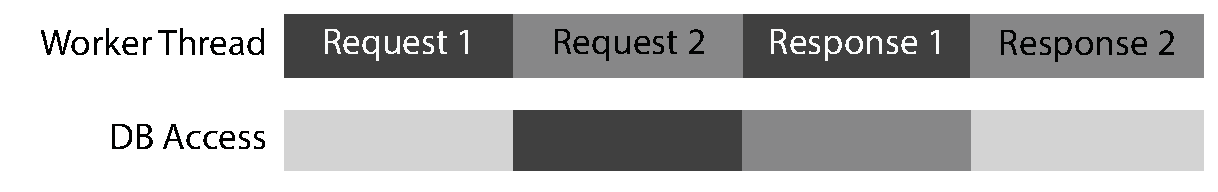
\includegraphics[width=.90\textwidth]{concurrency_2}
\caption{
A non-blocking scenario in a Web application. When request one (shown in dark grey) arrives, a database operation is necessary. This is a blocking operation, but since the worker thread does not have to wait for it to complete, the next request (shown in medium grey) can already be accepted and another database operation can be initiated. When the first database operation completes, the worker thread can send the response to the first client. Using more threads, this procedure can be heavily parallelised. 
}
\label{fig:concurrency_2}
\end{figure}

\begin{figure}
\centering\small
\begin{tabular}{c@{\hspace{12mm}}}
  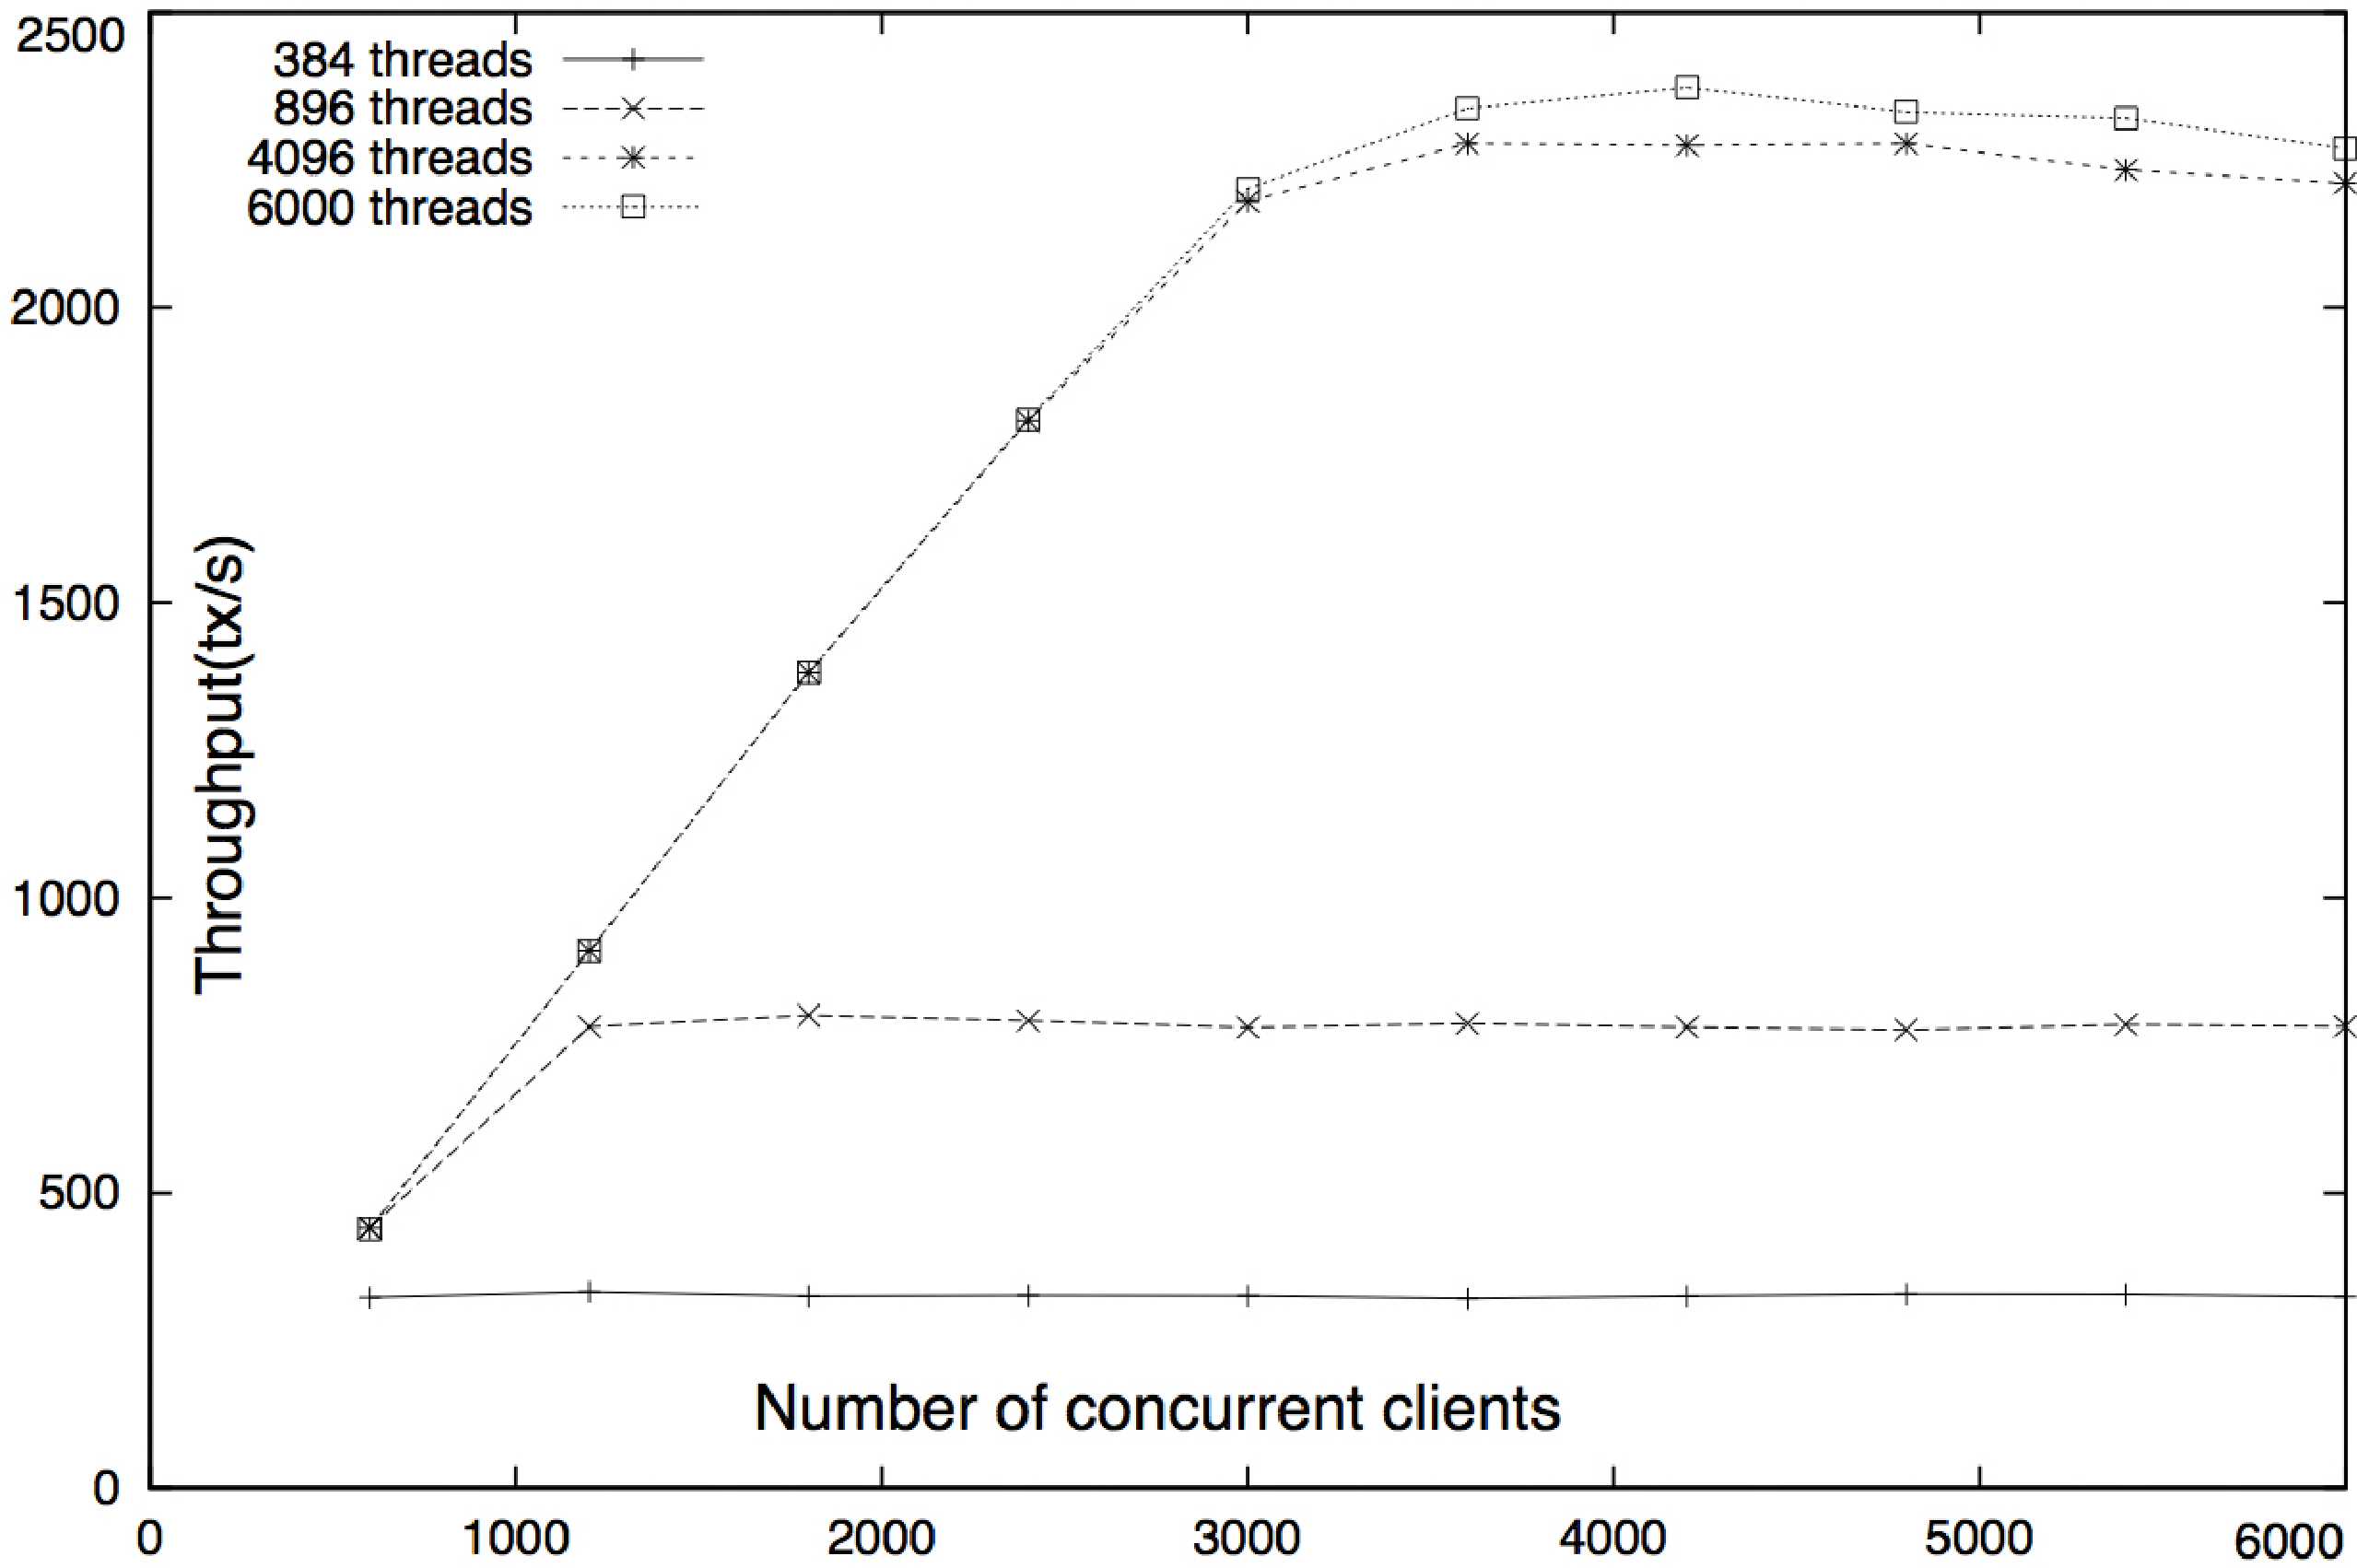
\includegraphics[width=.70\textwidth]{events_scale1} \\
  (a)
\\[14pt]
  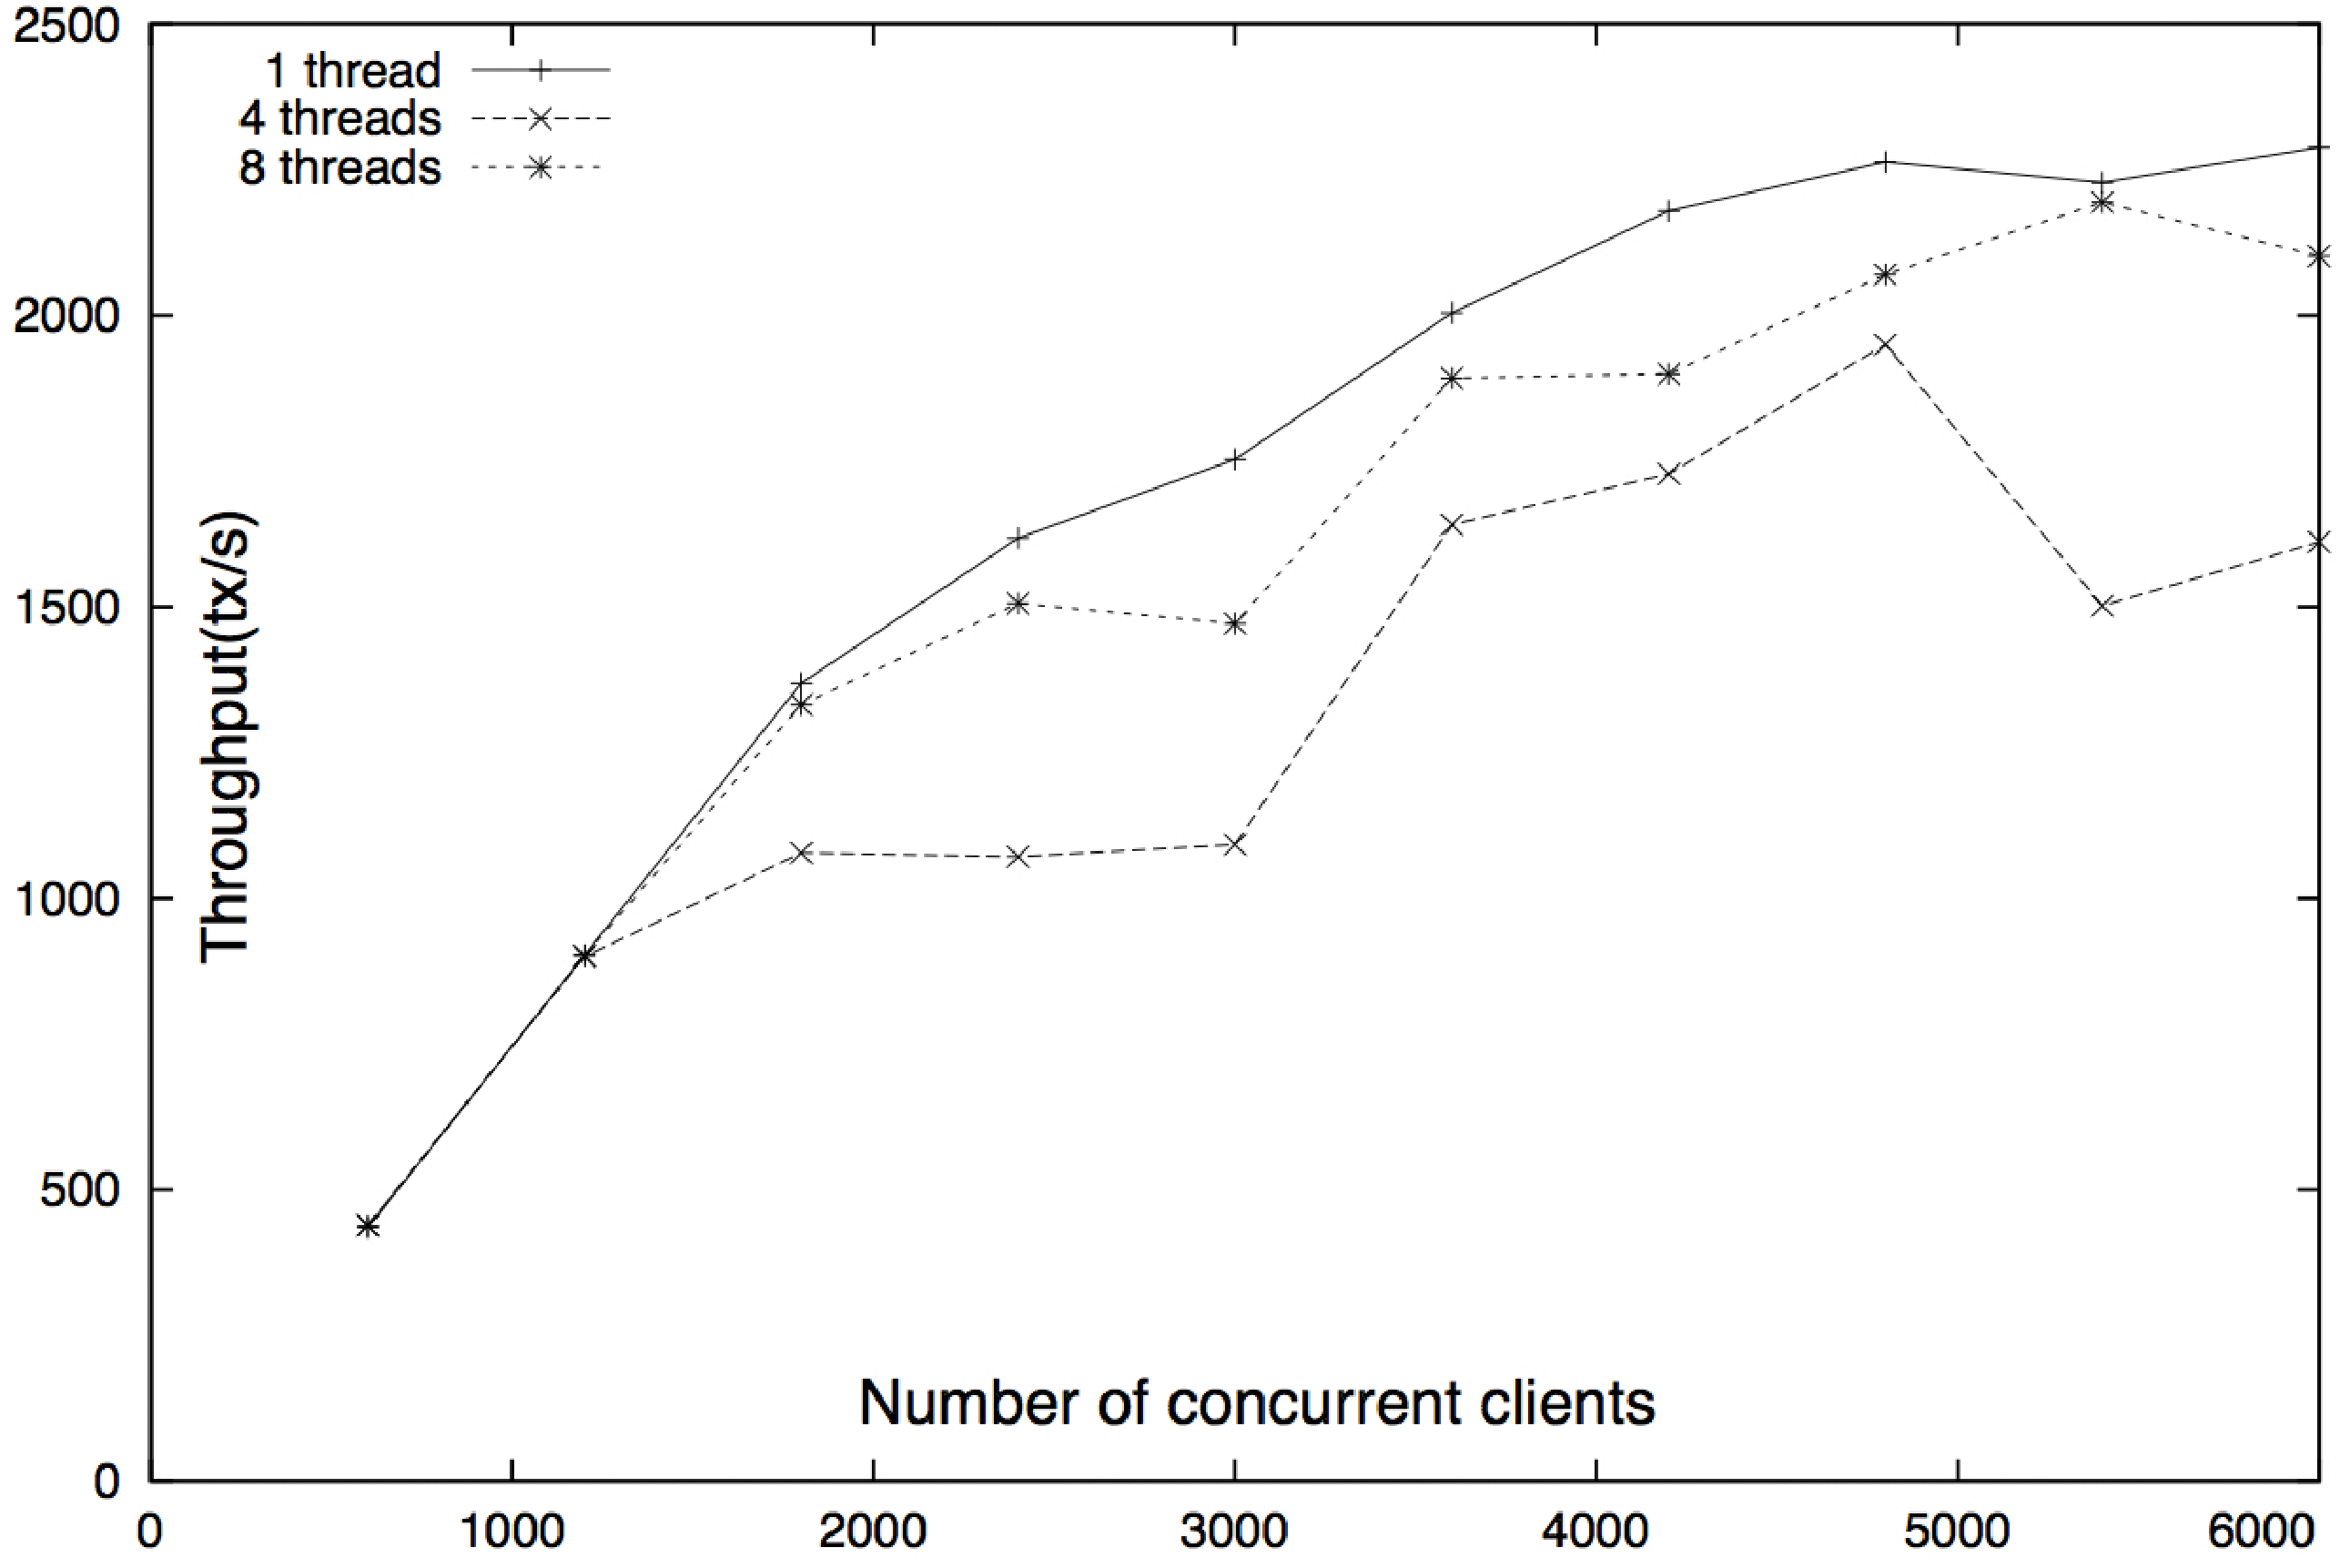
\includegraphics[width=.70\textwidth]{events_scale2} \\
  (b)
\end{tabular}
\caption{Typical scaling behaviours of a purely thread-based application and an event-based application. This example is taken from an experiment by D. Carrera et al. \cite{Carrera}. The graphs show the effect of an increasing number of clients (x-axis) on the request throughput (y-axis) using a standard \textit{httdp 2.0} Web server -- shown in (a) -- and using \textit{Java}'s event-based \textit{NIO} interface -- shown in (b). References: \textit{Apache httpd} (\url{http://httpd.apache.org/}), \textit{Java NIO} (\url{http://www.oracle.com/}). Image source: \cite{Carrera}.} 
\label{fig:events_scale}
\end{figure}
 
To scale a single event loop on one machine, one event loop process can be created for every processing core -- on a machine with a quad-core processor, four event loops can process incoming requests in parallel\footnoteref{lab:hyper}. In such on-system scaling situations, event-based systems have the advantage of reduced mutual exclusiveness of the program code, thus less locking situations tend to occur. An example for this is when a queue is accessed by multiple threads - only one thread can access the queue simultaneously, the other one has to wait.

Generally, it can be concluded, that for the specific scenario of a networking application like a Web server, event-based systems can provide more efficient performance and can thus be scaled more extensively with lower hardware requirements. Comparing figure \ref{fig:concurrency_1} and figure \ref{fig:concurrency_2}, it can be seen that given a blocking scenario like a database operation, event-based concurrency not only benefits the number of parallel requests, but can also lead to significant response time improvements.

\subsubsection*{Drawbacks}
Beside the implications of relinquishing the call stack pattern -- like flat program structure, more or less obfuscated flow of control and reduced state management capabilities -- there are other factors that have to be taken into account when using event-driven architectures: 

Due to the non-linear nature of an event-based system, \textit{race conditions} can occur. Race conditions typically happen, when the programmer expects a certain order of command execution, which are not guaranteed to be maintained under varying circumstances. For instance, if two Web requests are executed concurrently and the second response is expected to be always received after the first -- because it is supposed to trigger application logic that depends on the first response's data -- the application would fail if the responses would arrive out of order.

Additionally, event-based programs lack certain compiler optimisations\footnote{Compiling is the process of transforming a human-readable programming language into code that is better suited for execution by computers, e.g. binary code.} (given that the programming language used is compiled, rather than interpreted) like advanced memory management, inline functions\footnote{Function content is directly inserted into the code instead of calling the function reference multiple times. This leads to reduced execution time and memory overhead.} and compile-time warnings about race conditions \cite[p. 5]{Behren2003}.


\subsection{Staged Event-driven Architecture}
\label{sec:seda}
Staged event-driven architectures (short \textit{SEDA}) describe a special pattern of event-driven program flow that is rather different from the standard implementation (see section \ref{lab:events}) in certain aspects and can be to some amount considered the middle ground between purely thread-based and event-based architectures. The eponymous extension to traditional event-driven architecture is the presence of \textit{stages}, i.e. self-contained application components, each including an event queue and a comparably small, dynamically-sized thread pool (see figure \ref{fig:seda}). Additionally, each stage has monitoring and controlling agents that enable introspection of the application. This way, parameters like the number of threads in the thread pool and the batch size -- i.e. the number of events processed simultaneously in the stage -- can be dynamically adjusted by the application \cite{Welsh2001}. 

\begin{figure}
\centering\small
\setlength{\tabcolsep}{0mm}
  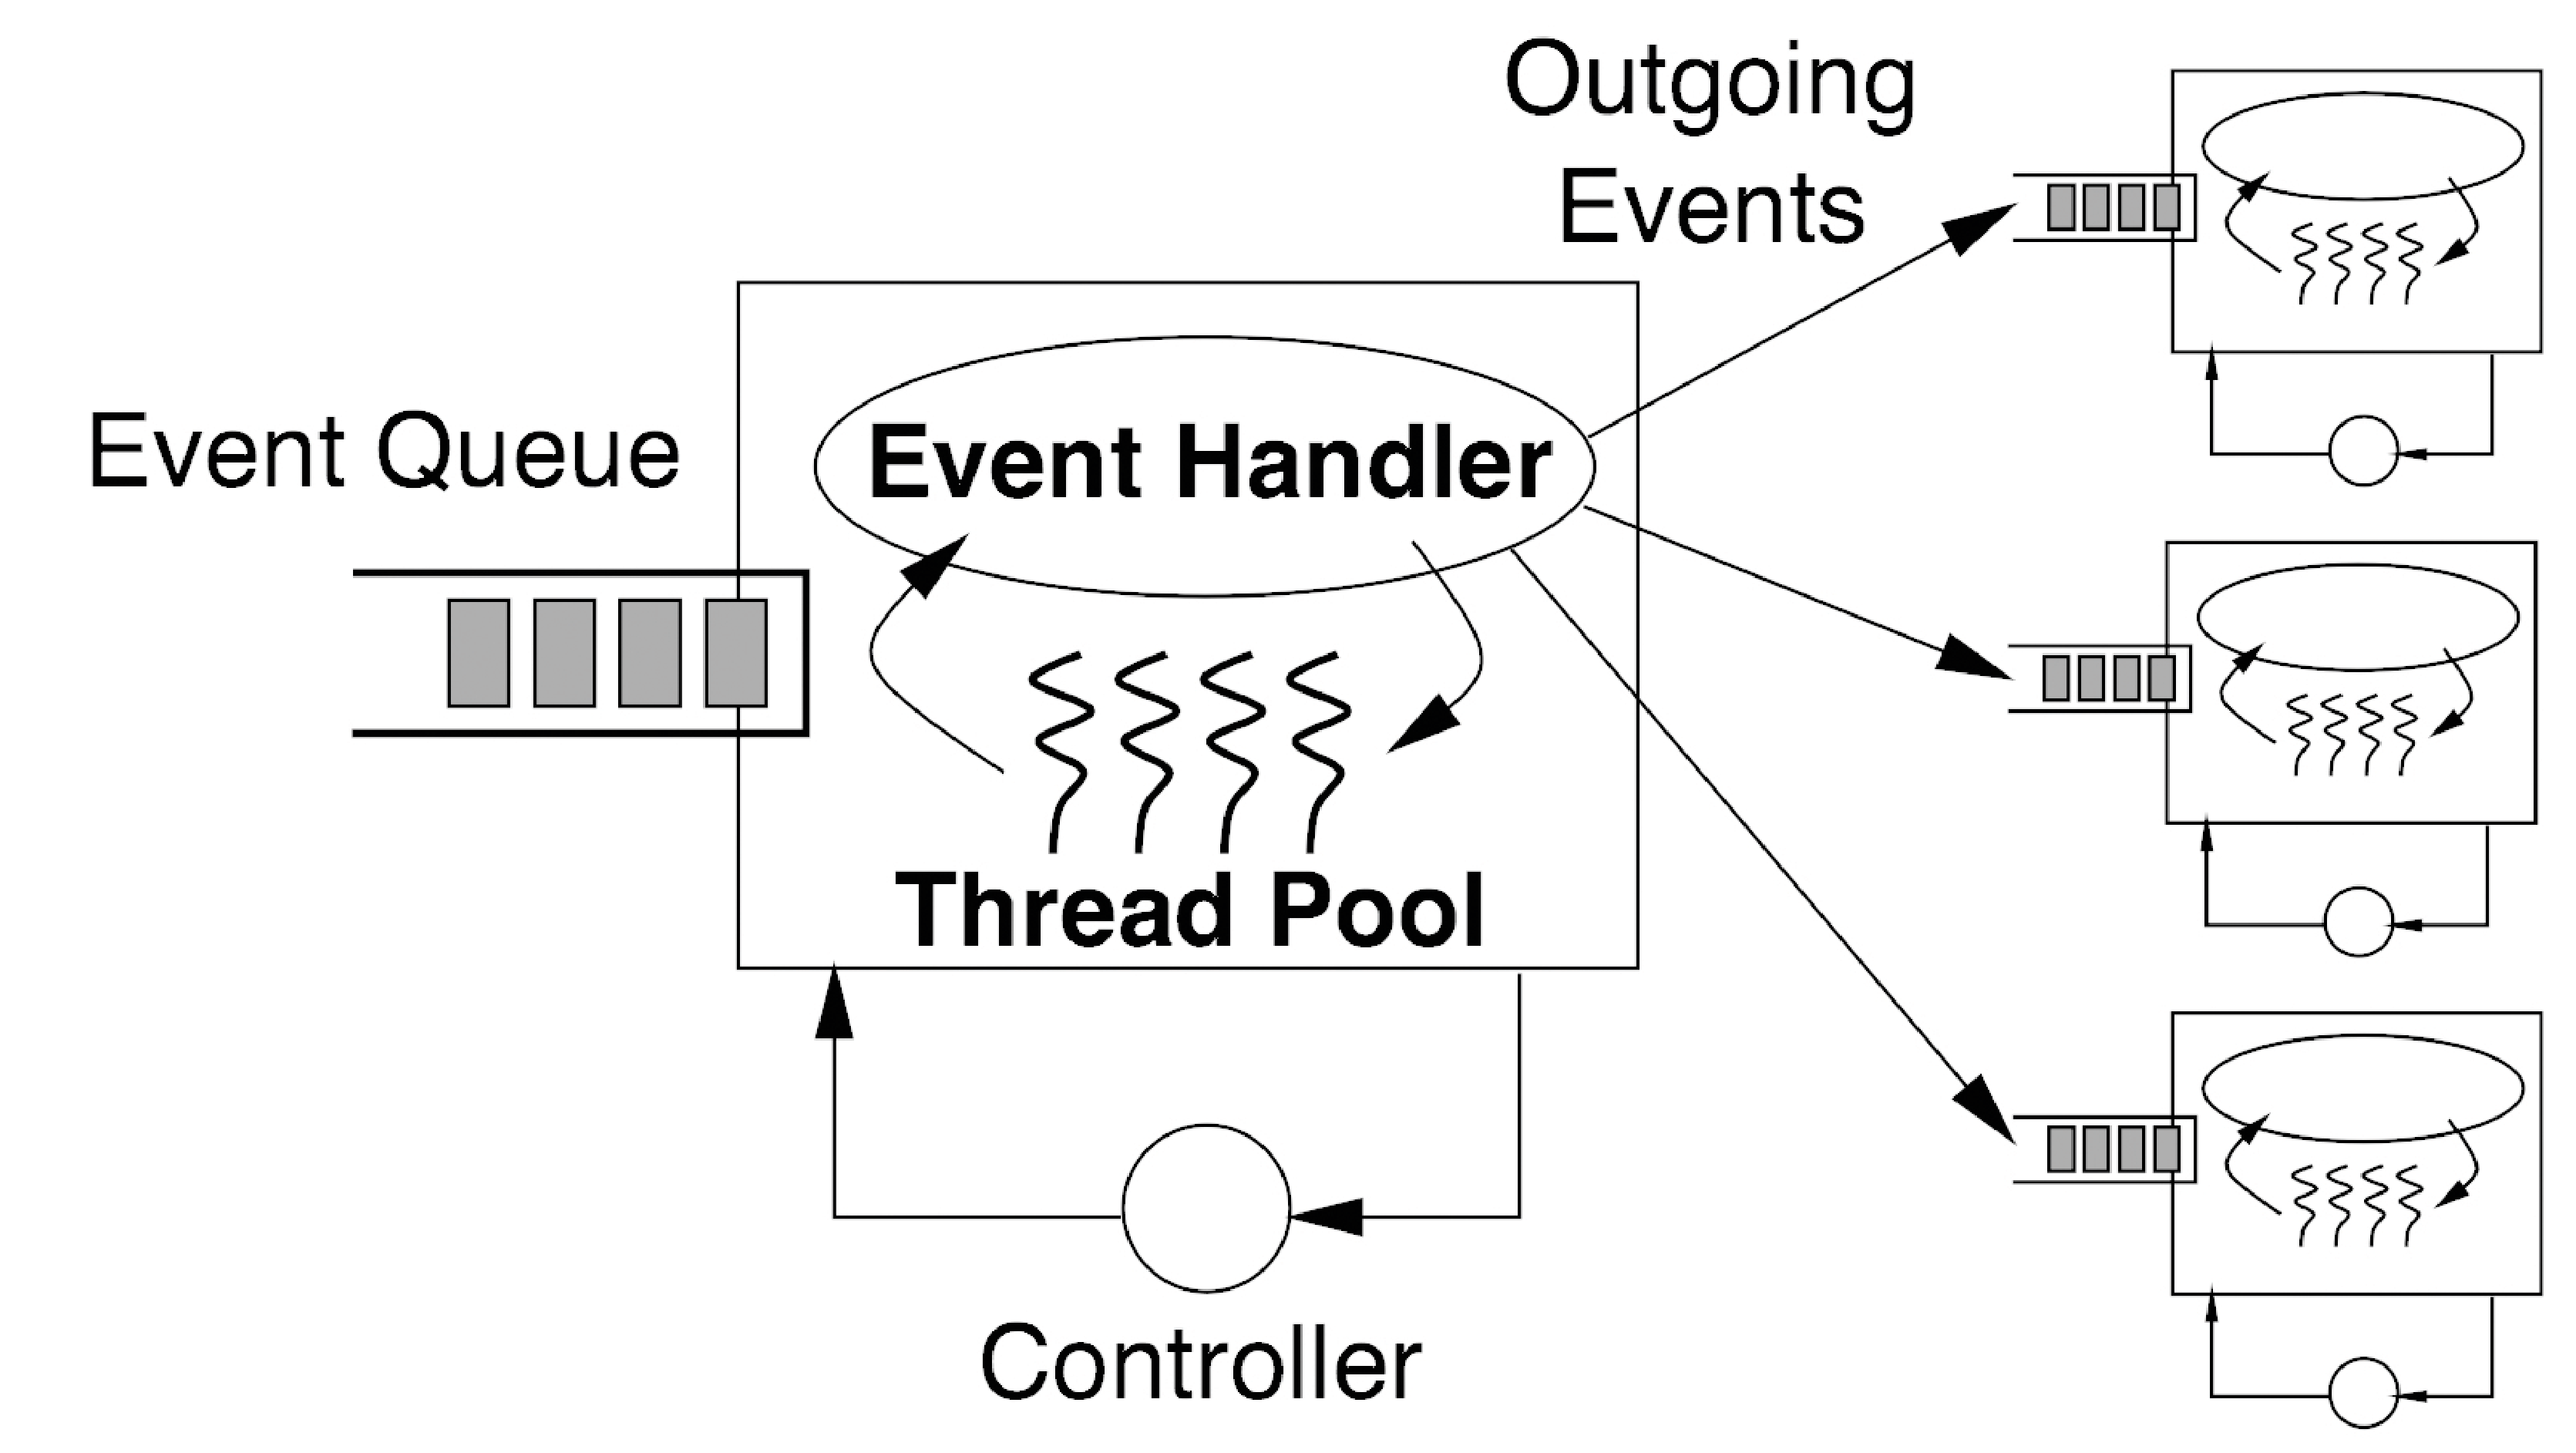
\includegraphics[width=.90\textwidth]{seda}
\caption{
Illustration of a single \textit{SEDA} stage (left) and the communication with other stages (right). Each stage has its own event queue, event handler, thread pool and resource controller. Image source: \cite{Welsh2001}
}
\label{fig:seda}
\end{figure}

\subsubsection*{Flow of Control}
This variation of application flow moderately reduces the effects of inversion of control introduced by event-driven architecture; an inherent advantage of this design is the introduction of modularity and structured flow of control. Another advantage of \textit{SEDA} is the adaptability to low-level operating system conditions like thread scheduling due to the aforementioned resource control elements; for instance, if less threads are available to a certain stage, the batch size can be reduced and thus the throughput can be maintained. Similar mechanisms can provide a certain level of explicit overload protection. An application that balances its own resources and changes its behaviour based on parameters like demand and response time is called a \textit{conditioned} application \cite{Welsh2001}. 

\subsubsection*{Drawbacks}
The coupling of stages by means of event queues is not necessarily supporting a clear application structure. M. Welsh, one of the developers mainly involved in the invention of \textit{SEDA} in 1999, states this coupling as a main problem of \textit{SEDA} \cite{seda}: 

\begin{quote}
If I were to design SEDA today, I would decouple stages (i.e., code modules) from queues and thread pools (i.e., concurrency boundaries). Stages are still useful as a structuring primitive, but it is probably best to group multiple stages within a single ``thread pool domain'' where latency is critical. Most stages should be connected via direct function call. I would only put a separate thread pool and queue in front of a group of stages that have long latency or nondeterministic runtime, such as performing disk I/O.
\end{quote}

Furthermore, due to the fact that every stage has its own thread pool, context switching overhead is generally considerably higher than in traditional event-based architectures \cite{seda}. Apart from that, queues tend to be an unsuitable data structure for high-concurrency applications, because they do not allow for concurrent access by multiple parties. Lastly, \textit{SEDA} requires a fair amount of fine-tuning on the part of the developer in order to function flawlessly \cite{event-architecture}.

\subsection{Actor Model}
\label{lab:actormodel}
In an actor-based architecture, \textit{actors} are the universal primitive of concurrent processing. An actor is an isolated (i.e. self-contained) entity that executes program logic. Actors can communicate with each other via asynchronous messages that can contain arbitrary data and a reference to the sender. Based on the nature of the received message, the actor can execute side-effect-logic like writing a file to disk, but can also send messages to other actors -- including the original sender. Actor-based architectures are similar to event-based architectures in the sense that both implement communication via message passing. The concept of a direct response like in all aforementioned architectural patterns -- be it via a call stack or a callback handler -- becomes irrelevant \cite{Haller2006}. 

\subsubsection*{Flow of Control}
Event-based architectures work by the principle of \textit{inversion of control} (see section \ref{lab:events}), which is a necessity given the intrinsic mechanisms of events. However, this limits the clearly defined structure of the program code and tends to be less idiomatic in nature. Message passing between actors, on the other hand, does not rely on inversion of control \cite{Haller2006}. Control remains solely with the sending actor, since he can decide, to whom -- if at all -- to send further messages (see figure \ref{fig:actor_flow}). This aids in reduced complexity when designing concurrent programs. Seen in this perspective, actor-based architectures can be seen as a compromise between thread- and event-based architectures.

Another aspect of actor-based program flow is that the loose coupling introduced by events is further extended. Instead of memorising references to the callee function, actors have the choice of sending a message back in order to create symmetric communication. Furthermore, an actor's internal state can only change in response to incoming messages -- there is no way of modifying actor state directly via methods or variables \cite[p. 38]{Haller2011}. This simple fact has great implications on state management across the application; this architectural characteristic is known as \textit{share-nothing} architecture \cite[p. 3]{Bonetta}.

\begin{figure}
\centering\small
\setlength{\tabcolsep}{0mm}
  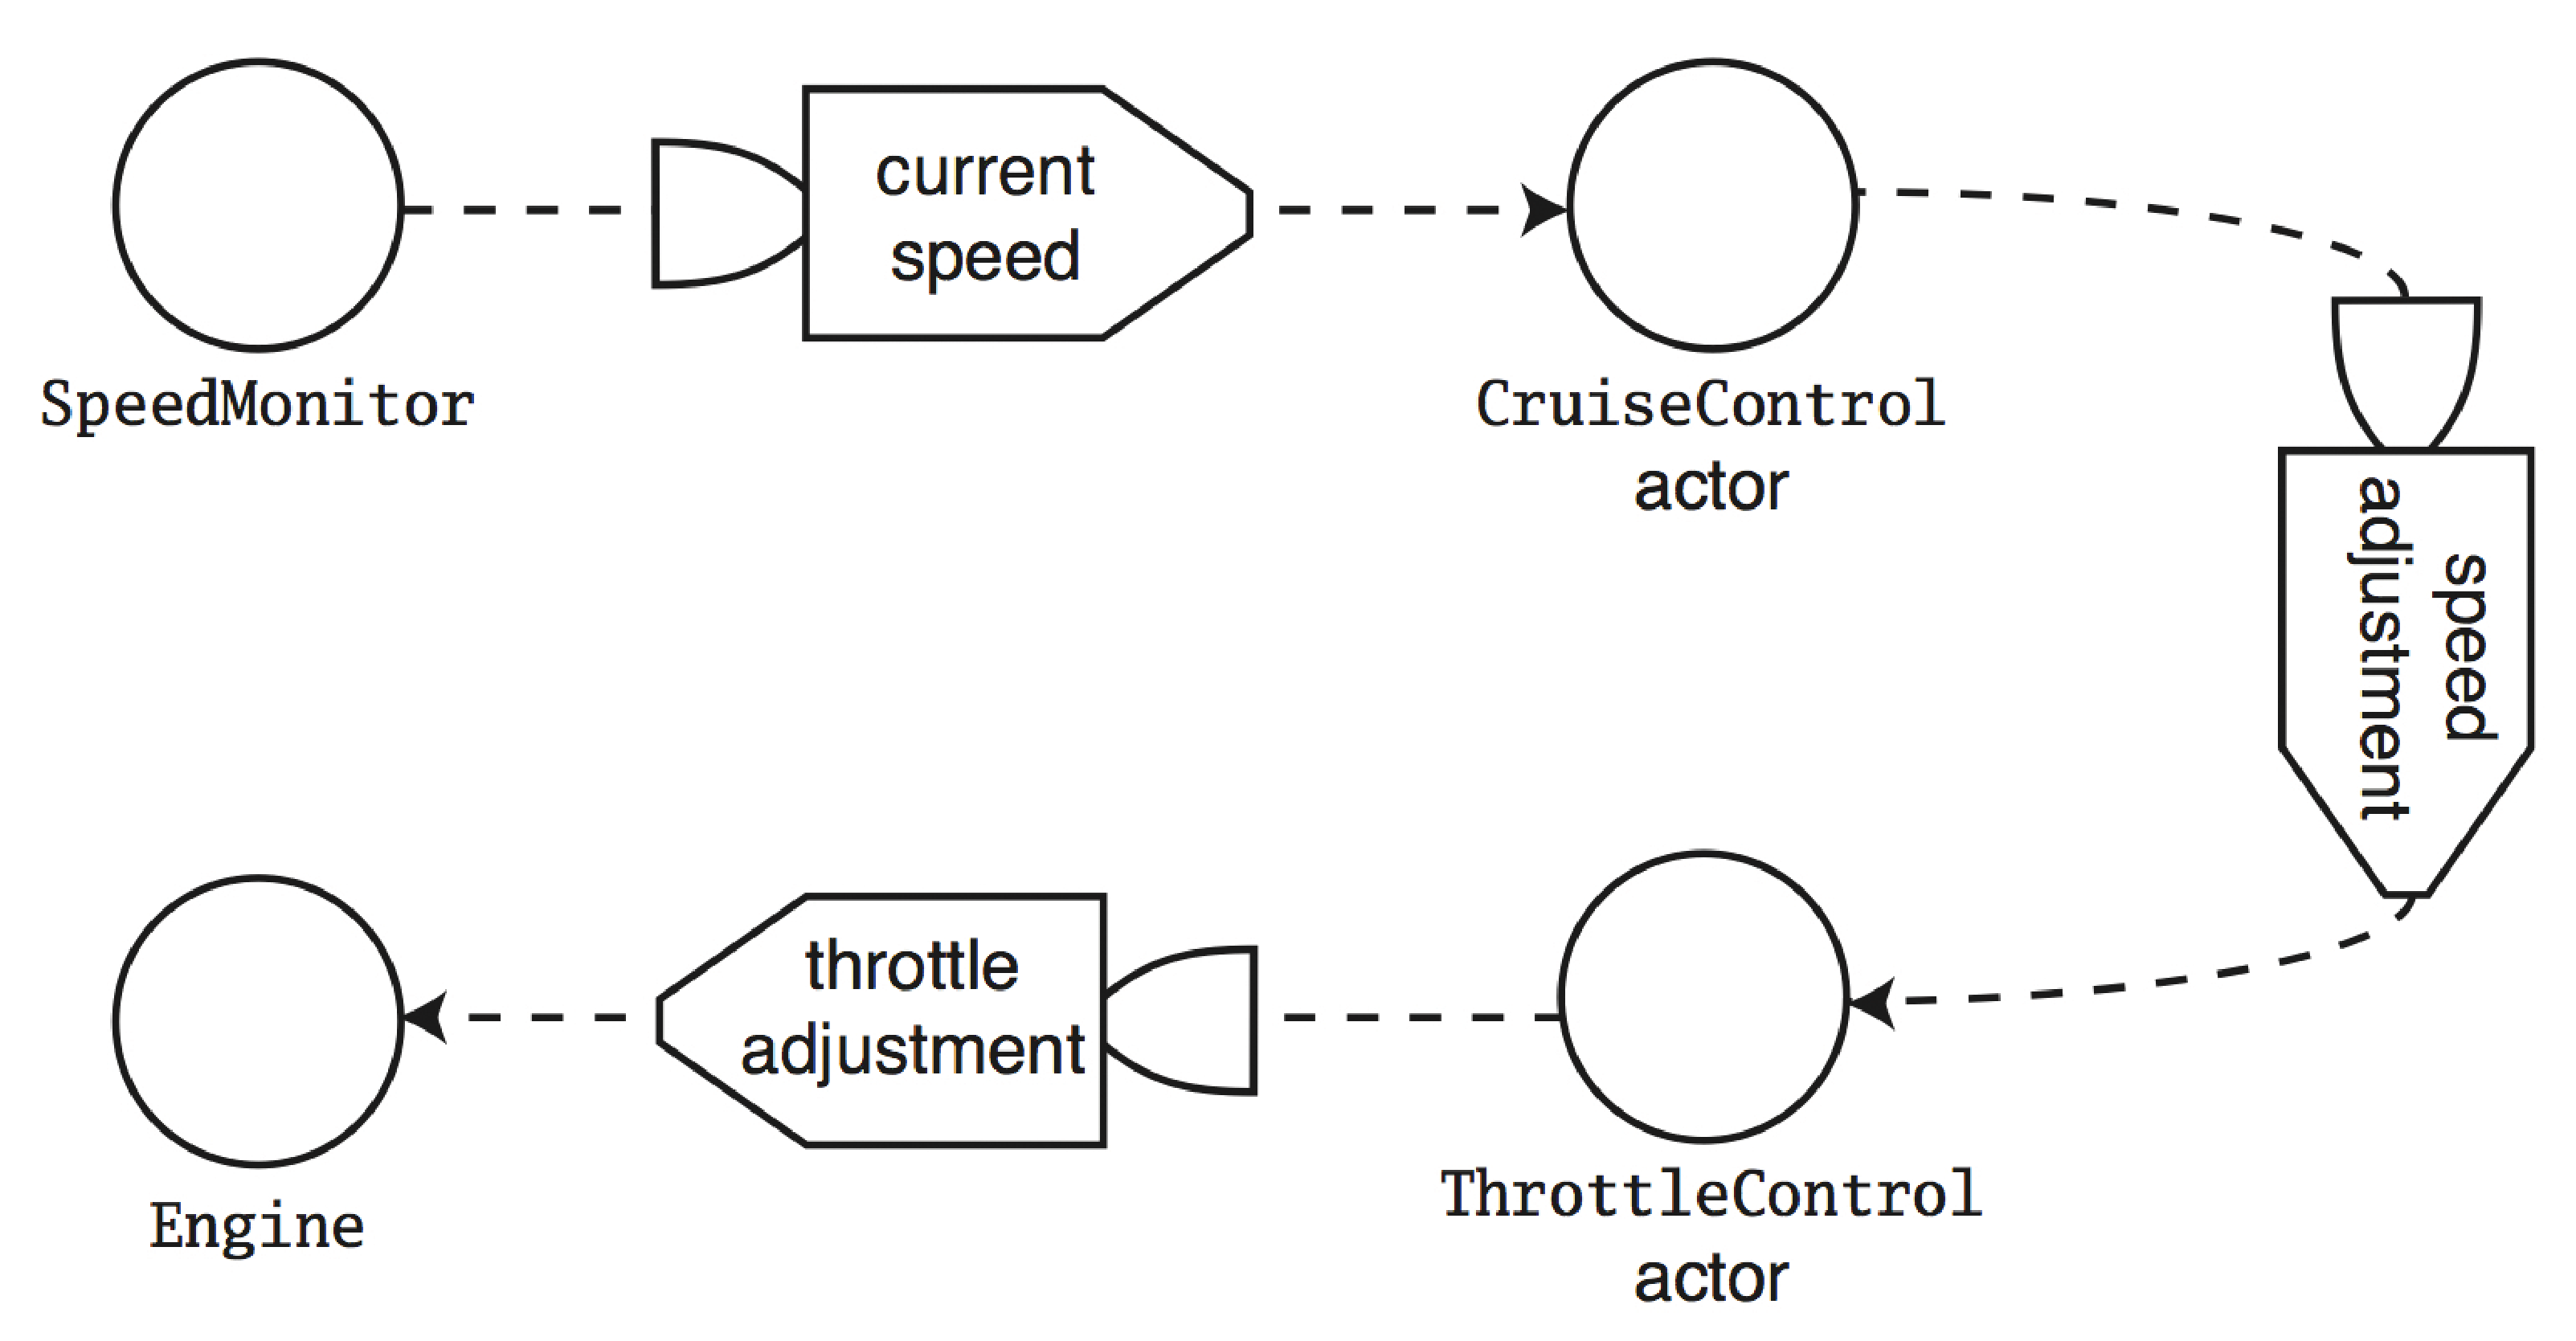
\includegraphics[width=.90\textwidth]{actor_flow}
\caption{
Illustration of an actor-based control flow. Actors are represented as circles and messages are represented as rockets. The speed monitor actor periodically sends a message containing the current speed to the cruise control actor. If a deviation of the desired speed is detected, an adjustment message is sent to the throttle control actor, who again sends a message to the engine. Image source: \cite{Haller2011}
}
\label{fig:actor_flow}
\end{figure}

Incoming messages are handled via \textit{mailboxes}, which are basically actor-specific queues that receive, filter and defer incoming messages. Like in event-based architectures, there is no guarantee in which order messages arrive in the mailbox and -- since the actor model does not specify a medium for passing messages (which may also be network-based, see below), a message can take arbitrarily long to reach its destination \cite[97]{Erb2012}. Since only the corresponding actor can access his mailbox and only one message is processed at a time, no concurrency issues -- like race conditions -- can arise for the actor state and the mailbox as well as in between messages \cite[p. 12]{Eriksson2013}. The orchestration of message processing is done by a \textit{dispatcher}, i.e. a part of framework logic that handles the execution of asynchronous, actor-based logic \cite[p. 97]{Gupta2012}. See figure \ref{fig:gil} for a basic illustration of resource mapping within an actor system.

\begin{figure}
\centering\small
\setlength{\tabcolsep}{0mm}
  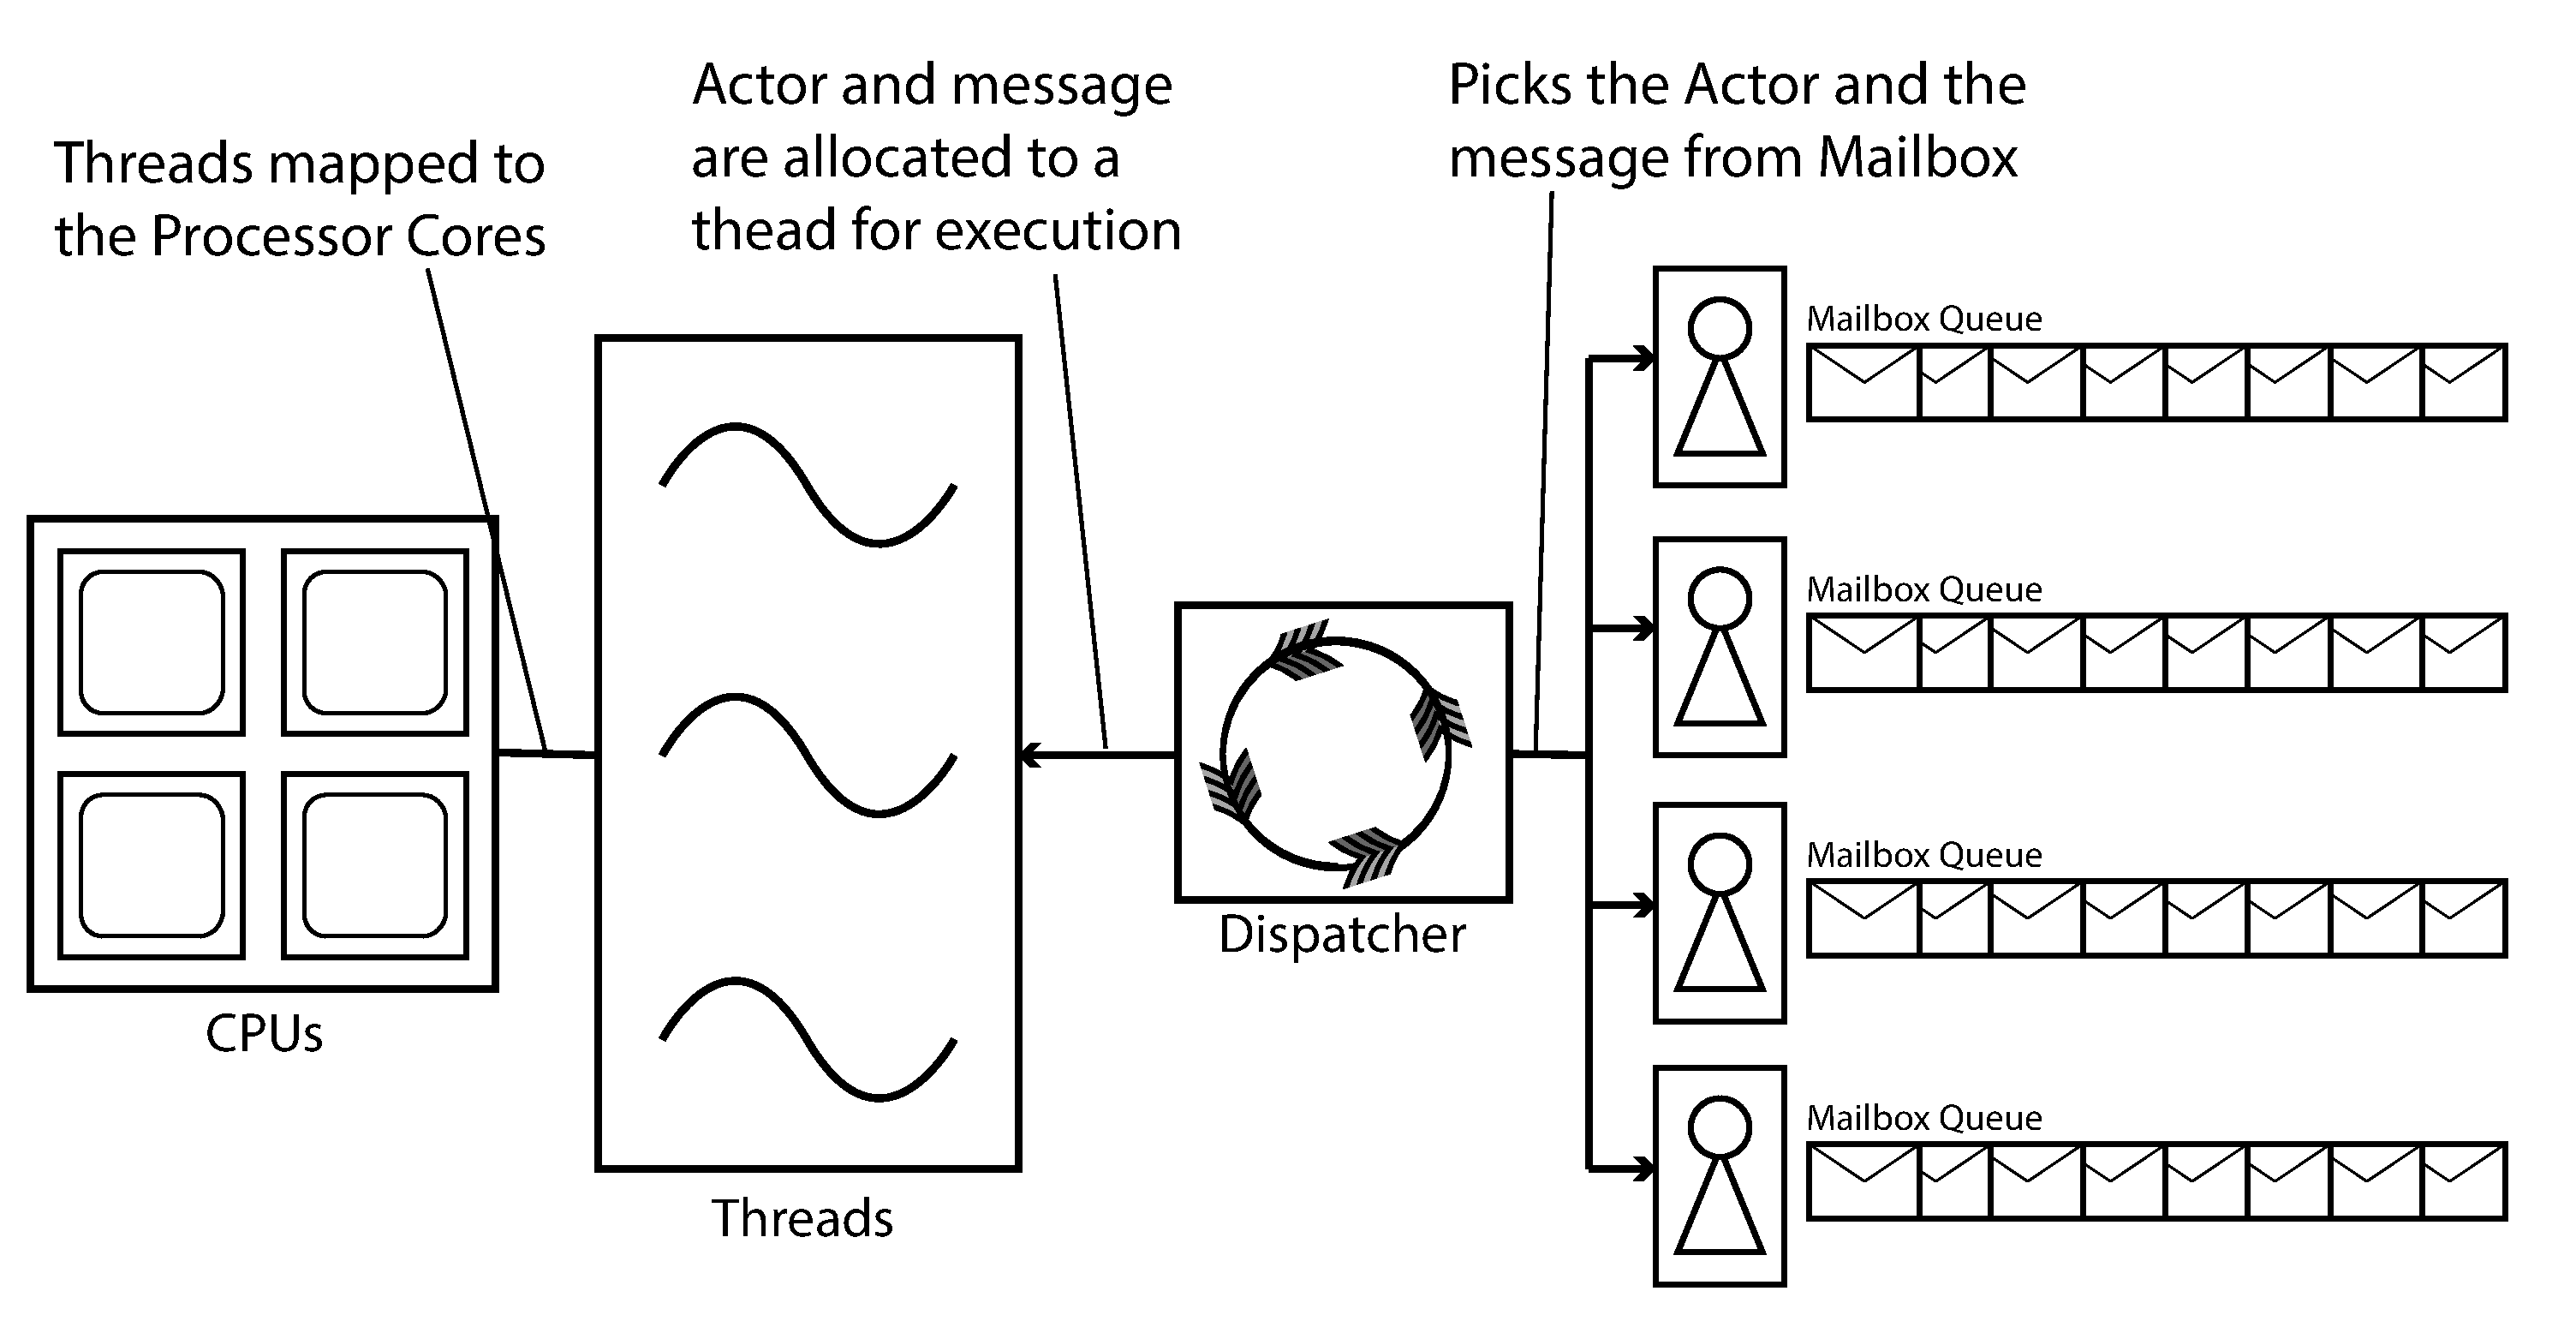
\includegraphics[width=.90\textwidth]{actors}
\caption{This graphic illustrates how resources are handled in a typical actor system. A \textit{dispatcher} distributes messages of actors to operating system threads based on certain strategies (e.g. load balancing). Image source: \cite{Gupta2012}}
\label{fig:gil}
\end{figure}

Actors are also \textit{resilient}, i.e. robust in the case of failure. \textit{Erlang}, one of the programming languages first to embrace the actor model, coined the term \textit{let-it-crash}; due to the isolated nature of actors, one actor unable to proceed working (i.e. \textit{crashing}) will not affect other actors. The actor model also supports hierarchical structures of actors, which enable supervising actors to restart crashed actors \cite{Armstrong2007}.

\subsubsection*{Scalability}
Due to the lightweight nature of actors, they can be used in abundance on single systems. P. Haller and M. Odersky state that 5000 concurrently active threads can support over 1200000 concurrent actors \cite[p. 2]{Haller2009}. Moreover, due to their \textit{share-nothing} nature, actors are not limited to one physical system, but work as well on distributed and replicated systems \cite[p. 233]{Gupta2012}. This makes the actor model by far the most scalable of all models listed herein. 

\subsubsection*{Drawbacks}
The practice of relinquishing shared state and using immutable messages for communication reduces the risk of problems inherent to high concurrency -- like race conditions and deadlocks -- but does not eliminate them. Furthermore, inconveniences arise when a specific execution order is crucial; while event-based architectures provide \textit{callback functions} to handle this situation, guaranteeing execution order within actor-based architectures is non-trivial. What's more is that actors do not provide any means of object orientation or inheritance \cite{Mackay97}. Also, like in event-based architectures, there is no additional compiler support (see section \ref{lab:events}).
